\documentclass[11pt]{article}

\usepackage{times}
\usepackage{amsbsy}

\usepackage{geometry}                % See geometry.pdf to learn the layout options. There are lots.
\geometry{letterpaper}                   % ... or a4paper or a5paper or ... 
%\geometry{landscape}                % Activate for for rotated page geometry
%\usepackage[parfill]{parskip}    % Activate to begin paragraphs with an empty line rather than an indent
\usepackage{graphicx}
\usepackage{amssymb}
\usepackage{epstopdf}

\DeclareGraphicsRule{.tif}{png}{.png}{`convert #1 `dirname #1`/`basename #1 .tif`.png}

\newcommand{\be}{\begin{equation}}
\newcommand{\ee}{\end{equation}}
  
\newcommand{\beq}{\begin{eqnarray}}
\newcommand{\eeq}{\end{eqnarray}}
\newcommand{\ba}{\begin{eqnarray}}
\newcommand{\ea}{\end{eqnarray}}

\newcommand{\ua}{{\bf u}_\alpha}
\newcommand{\utwo}{\overline{\bf u}_2}


\newcommand{\ubar}{\overline{u}}
\newcommand{\vbar}{\overline{v}}
\newcommand{\phis}{{\phi}^{*}}
\newcommand{\thetas}{{\theta}^{*}}

\title{ {\bf NearCoM-TVD}\\
A Hybrid TVD Solver for Nearshore Community Model  \\
Documentation and User's Manual \\
( DRAFT)}
\author{Fengyan Shi, James T. Kirby, Tian-Jian (Tom) Hsu and  Jianlin Chen \\
Center for Applied Coastal Research, University of Delaware, Newark, DE 19716}

\date{\today}   
                                   
\begin{document}

\maketitle


\vspace*{8cm}
     
\begin{center}

{\Large 
Center for Applied Coastal Research \\ University of Delaware \\
Research Report NO. CACR-11-XX}
\end{center}     
\thispagestyle{empty}

\newpage
\begin{center}{\bf \Large Acknowledgements}
\end{center}

\vspace*{0.5cm}
  This model development  was  sponsored  by  
 the Office of Naval Research, Coastal Geosciences Program through grant N00014-10-1-0406, Delaware Sea Grant RHCE1 and NOAA BOEMRE No. M10PG00236.

\thispagestyle{empty}

\newpage
\begin{abstract}

The report documents a new version of the Nearshore Community  Model (NearCoM) initially developed during the National Oceanography Partnership Program (NOPP). The model couples a wave model SWAN, a nearshore circulation model SHORECIRC and a sediment model in a fully parallelized computational environment.
The wave module SWAN is modified based on the structured grid Version 40.51AB, which is the last stable version before the release of the unstructured grid version UnSWAN. The circulation module SHORECIRC is improved numerically using  a hybrid TVD solver. The sediment module uses two optional sediment transport formulas. One is  Sousby's formula (Soulsby, 1997) which takes into account total load sediment transport by both waves and currents. 
The other option for sediment transport is Kobayashi et al's (2007) formula which was initially used in the CSHORE one-dimensional model and was modified for two-dimensional applications. 
This development emphasizes numerical improvements, including 
1) a conservative form of SHORECIRC equations in non-orthogonal curvilinear coordinates; 2) MUSCL-TVD solver with adaptive Runge-Kutta time stepping;  3) wetting-drying moving boundary condition with incorporation of HLL construction method into the scheme; 4) fully parallel computation with equal CPU load for each processor.  
The documentation provides derivations of the conservative form of theoretical equations in generalized curvilinear coordinates, re-arrangement of pressure gradient term in order to obtain a numerically well-balanced form, detailed numerical schemes, users' manual and examples.

\end{abstract}

\thispagestyle{empty}

\newpage

\begin{center} 
 \tableofcontents 
\end{center}

 \newpage
 
 \listoffigures
 
 \newpage
 
% \listoftables
 
 \newpage


\addcontentsline{toc}{subsection}{}

\newpage



\section{Introduction}

The Nearshore Community Model System, NearCoM, was developed during the National Oceanography Partnership Program (NOPP),  for predicting waves, currents, sediment transport and bathymetric change in the nearshore ocean. The modeling system consists a suite of `modules', each of which handles a focused subset of the physical processes being studied.  A master program (Shi et al., 2005) is used to link those modules (usually integration of three modules: wave, circulation and seabed) and to handle data input, output and internal data transfer between modules. The NearCoM system provides various wave, circulation and sediment modules based on different theories and numerical mechods, which can be configured and extended by users themselves.  A frequently-used example of NearCoM is a combination of a wave module REF/DIF-1 (Kirby and Dalrymple, 1992 ), circulation module SHORECIRC (Svendsen, et al., 2003) and sediment module HH (Haas and Hanes, 2004). An application of coupling a wave module and a 3-D circulation module (POM) has been reported recently by Newberger and Allen (2007). 

Because NearCoM focuses on predicting nearshore waves and wave-induced nearshore processes,
modules in the original NearCoM system were developed specifically for nearshore applications, basically between
the shoreline and about 10 m water depth. There are difficulties that limit the general application of 
NearCoM  to some ocean-exposed coastal regions. For example, in tidal inlet regions, the tidal forcing is
not considered in the model because of unknown tidal boundary conditions; wave input is somewhat arbitrary
as there is no link to a large- scale wave generation and transformation model which could predict spatial inhomogeneities
in incident wave conditions; and sediment transport processes may also need boundary conditions
associated with offshore sediment sources or river discharges.
Most recently, Shi et al. (2011) integrated the wave model SWAN and a modified version of  SHORECIRC in the system to extend its application to 
a large-scale beach-inlet system.  

In the aspect of numerics, there have been several improvements in numerical approaches for SHORECIRC since it was  released. The original version of SHORECIRC is based on SHORECIRC equations in Cartesian coordinates and implemented using  finite difference schemes in which time stepping is treated by the predictor-corrector scheme, while spatial differencing is handled by a second-order central differencing scheme. A curvilinear version of SHORECIRC was developed based on a coordinate transformation from Cartesian to a generalized curvilinear grid system (Shi et al., 2003). The curvilinear SHORECIRC was further enhanced using  a CFL-free numerical scheme in order to improve computational efficiency (Shi et al., 2007). 

There is a growingly demand recently  to use NearCoM in various coastal applications, such as wave-current interaction in an inlet system, storm-induced coastal inundation, beach and dune erosions, tidal flat processes, and etc. Some large-scale processes  such as tides, wind  and wind-wave generation play important roles in those applications. Those applications raise concerns about model efficiency and stability in a long-time simulation.  
Although the recent version with a CFL-free numerical scheme is efficient in terms of a large time step, there is an 'ADI effect' caused by an extreme large Courant number (Casulli and Cheng,1992). 
The computational codes for all versions of SHORECIRC are based on serial computation using a single computer processor. 

In this work, we developed a new code of SHORECIRC using a hybrid method combining the finite-volume and finite-difference --- TVD-type scheme (Toro, 2009). This scheme has been proved to be  stable and robust in modeling wave breaking and moving shorelines in the most recent development of the fully-nonlinear Boussinesq model with a TVD solver (FUNWAVE-TVD, Shi et al., 2011a, 2011b, Tehranirad et al., 2011, Kirby et al., 2011).  Good performance of the TVD scheme was  also found in several Boussinesq and shallow water equation models developed by other recent authors (Tonelli and Petti, 2009, Roeber et al., 2010, Shiach and Mingham, 2009, Erduran et al., 2005, and others).

A conservative form of SHORECIRC equations was derived in order to use the hybrid numerical scheme. The surface elevation gradient term was rearranged following Shi et al. (2011) to obtain a numerically well-balanced form.    In contrast to previous  temporal schemes, which usually require uniform time-stepping, we used adaptive time stepping based on the  Runge-Kutta method.  
In the hybrid spatial scheme,  a MUSCL reconstruction technique, which is accurate up to the fourth-order,  was used in the Riemann solver.  

The wave model SWAN,  the circulation model SHORECIRC and the sediment module  are integrated as a single model in the same parallelized model framework. The domain decomposition technique, with the Message Passing Interface (MPI),  is used for the SHORECIRC code  in connection with the decomposed SWAN grid through global mapping.  The parallel scheme has a feature of equal CPU load for each processor, which is more efficient in contrast to the recent model coupling framework of WRF, SWAN and ROMS by Warner et al. (2008) who uses the Model Coupling Toolkid (MCT) to distribute CPUs unevenly for each processor. 

This report  provides derivations of the conservation form of theoretical equations with a well-balanced pressure gradient term, numerical schemes, and users' manual. The last part of report  uses an idealized case to demonstrate basic model setup for a general application, and  illustrates some model applications to  problems of wave-induced nearshore circulation. 


\section{Theory}

\subsection{SHORECIRC equations}
SHORECIRC is a quasi-3D nearshore circulation model for prediction of wave-induced nearshore circulation. It is a 2D horizontal model which incorporates the effect of the vertical structure of horizontal flows.  In Putrevu and Svendsen (1999), the instantaneous horizontal velocity is split as
\be
u^{ins}_\alpha = u^{\prime}_{\alpha} + u_{w \alpha} + u_\alpha + u_{1 \alpha}
\ee
wherer $u^{\prime}_{\alpha}, u_{w \alpha}, u_\alpha$ and $u_{1 \alpha}$ are, respectively, the turbulence component, the wave component, the component of depth-averaged and short-wave-averaged velocity, and the vertical variation of the short-wave-averaged velocity. 
The complete SHORECIRC equations can be expressed  in the Cartesian form as in Svendsen et al. (2003) or in the curvilinear form in Shi et al. (2003). In this section, we derive a conservative form of the equations in generalized curvilinear coordinates in order to use the TVD numerical scheme. 

SHORECIRC equations in Cartesian coordinates $(x_1, x_2)$ can be expressed as

\be
\frac{\partial \eta}{\partial t} + \frac{\partial Hu_\alpha}{\partial x_\alpha} =0
\ee
\be
\frac{\partial H u_\alpha}{\partial t} + \frac{Hu_\alpha u_\beta}{\partial x_\beta} +f_\alpha+ g H \frac{\partial \eta}{\partial x_\alpha} + \frac{1}{\rho} \frac{\partial T_{\alpha \beta}}{\partial x_\beta} + \frac{1}{\rho} \frac{\partial S_{\alpha \beta}}{\partial x_\beta}  + \frac{\tau^b_\alpha}{\rho} - \frac{\tau^s_\alpha}{\rho} + \mbox{ROT} = 0
\label{mom_cart}
\ee
where $\eta$ represents the wave-averaged surface elevation, $H = \eta + h$,  in which $h$ is still water depth. The depth-averaged and wave-averaged velocity $u_\alpha$ is defined by the `Lagrangian' averaging as
\be
u_\alpha = \frac{1}{H} \overline{\int_{-h}^\zeta u^{ins}_\alpha}
\ee 
where $\zeta$ is the instantaneous surface elevation. This split is different from Haas et al. (2003) who used the `Eulerian' concept for their split. For the Lagrangian averaging method, it is assumed that
\be
  \int_{-h}^\eta u_{1\alpha} dz = - Q_{w \alpha}
\ee
where $Q_{w \alpha}$ is the short wave flux. 

In (\ref{mom_cart}), $f_\alpha$  represents the Coriolis force which was not considered in the previous SHORECIRC equations (Putrevu and Svendsen, 1999). $T_{\alpha \beta}, S_{\alpha \beta}, \tau^s_\alpha$ and  $\tau^b_\alpha$ are the depth-integrated Reynolds' stress, the wave-induced radiation stress (Longuet-Higgins and Stewart, 1962, 1964), the surface shear stress and the bottom shear stress, respectively.   ROT represents the rest of terms associated with 3D dispersion terms which are not presented here because they do not involve the coordinate transformation conducted below. Interested readers are referred to Putrevu and Svendsen (1999).

A curvilinear coordinate transformation is introduced in the general form

\be
\xi^1 = \xi^1 (x_1,x_2), \ \ \ \   \xi^2 = \xi^2 (x_1,x_2)
\ee
where $(\xi^1, \xi^2)$ are the curvilinear coordinates. We use superscript indices, i.e.,  $()^\alpha$, to represent the contravariant component and subscript indices for the Cartesian component  of a vector.  The relation between the Cartesian component $u_\alpha$ and the contravarient component $u^\alpha$ can be written, by definition, as
\be
u^\alpha = u_\beta L^\alpha_\beta
\ee
where
\be
L^\alpha_\beta = \frac{\partial \xi^\alpha}{\partial x_\beta}
\ee
Using the chain rule, the derivative of a function $F$ with respect to $x_\alpha$ in the Cartesian coordinates can be expressed in the curvilinear coordinates $\xi^\alpha$ by
\be
\frac{\partial F}{\partial x_\alpha} = L^\beta_\alpha \frac{\partial F}{\partial \xi^\beta}
\label{der}
\ee
Using the metric identity law (Thompson et al., 1985):
\be
\frac{\partial}{\partial \xi^\alpha}(J L^\alpha_\beta) \equiv 0
\label{identity}
\ee
 (\ref{der}) can be rewritten in a different form as
\be
\frac{\partial F}{\partial x_\alpha} = \frac{1}{J} \frac{\partial F J L^\beta_\alpha}{\partial \xi^\beta}
\label{der2}
\ee
Using (\ref{der2}), the conservative form of SHORECIRC equations in curvilinear coordinates can be derived as

\be
\frac{\partial \eta}{\partial t} + \frac{1}{J}\frac{\partial J P^\alpha}{\partial \xi^\alpha} = 0
\label{mass1}
\ee

\ba
\nonumber
\frac{\partial Hu_\alpha}{\partial t} + \frac{1}{J} \frac{\partial }{\partial \xi^\beta} \left[ JP^\beta u_\alpha  +\frac{1}{2} g (\eta^2 +2 \eta h)  J L^\beta_\alpha \right] +f_\alpha -  g \eta \frac{1}{J}  \frac{\partial }{\partial \xi^\beta} (h J L^\beta_\alpha)  \\
+ \frac{1}{\rho} \frac{1}{J}  \frac{\partial }{\partial \xi^\gamma} (S_{\alpha \beta} J L^\gamma_\beta) 
+ \frac{1}{J}  \frac{\partial }{\partial \xi^\gamma} (\tau_{\alpha \beta} JHL^\gamma_\beta)
+ \frac{\tau^b_\alpha}{\rho} - \frac{\tau^s_\alpha}{\rho} + \mbox{ROT} = 0 
\label{conserv1}
\ea
Note that  equations (\ref{mass1}) and (\ref{conserv1}) contain both the Cartesian and  contravariant variables, which are different from the contravariant-only form in Shi et al., (2003). A difficulty in deriving the conservative form of the momentum equations using contravariant-only variables has be noticed by several authors (e.g., xxx) in shallow water applications.   
 Here, we follow Shi and Sun (1995) who used both Cartesian and contravariant variables in the derivation of the momentum equations. 
 
  In (\ref{mass1}) and (\ref{conserv1}), 
 $P^\alpha = H u^\alpha$, denotes the contravariant component of volume flux,  the Coriolis force $f_\alpha$ uses the Cartesian components, i.e., $(-f H v,  fH u)$, $S_{\alpha \beta}$ represents the Cartesian component of radiation stress. In the present application, the gradient of radiation stresses  (the fifth term of (\ref{conserv1})) is obtained directly from the wave module SWAN.    $\tau_{\alpha \beta}$  represents the Cartesian component of turbulent shear stress, $\tau^b_\alpha$ and $\tau^s_\alpha$ are the Cartesian components of bottom stress and wind stress.  


In the derivation of the momentum equations, the surface gradient term is treated following Shi et al. (2011) who reorganized this term in order to make it well-balanced in a MUSCL-TVD scheme for a general order.  The  expression in curvilinear coordinates can be written as
\be
-gHJ\frac{\partial \eta}{\partial x_\alpha} = -\frac{\partial }{\partial \xi^\alpha} \left [\frac{1}{2} g (\eta^2 +2 \eta h) J L^\alpha_\beta \right] + g \eta \frac{\partial }{\partial \xi^\alpha} (h J L^\alpha_\beta)
\ee

There are several advantages in using equations (\ref{mass1}) and (\ref{conserv1}) versus the contravariant-only form in Shi et al. (2003). First, they are a conservative form which can be implemented  using a hybrid numerical scheme. Second, all forcing terms resume to a vector form  in Cartesian coordinates in contrast to the contravariant form in Shi et al. (2003). Third, 
the radiation stress term $S_{\alpha \beta}$ uses the original form defined in Cartesian coordinates, thus that  there is no need to make a transformation for the second-order tensor.  The disadvantage is that (\ref{conserv1}) contains both the Cartesian component $u_\alpha$ and the contravariant component $P^\alpha$. However, in terms of the hybrid numerical  scheme used in the study, it is convenient to solve both of the two variables using the explicit numerical scheme, rather than  the implicit numerical scheme used  in Shi et al., (2007).

%The treatment of turbulent shear stress terms follows the scheme for the radiation stress terms. The extended form of the shear stress terms can be found in Appendix A. $\tau_{\alpha \beta}$ is defined in the Cartesian coordinates as
%\be
%\tau_{\alpha \beta} = \nu_t \left ( \frac{\partial u_\alpha}{\partial x_\beta} + \frac{\partial u_\beta}{\partial x_\alpha} \right)
%\label{shear}
%\ee
%The derivatives in the Cartesian coordinates are calculated using (\ref{der1}). 



 Wind stress in SHORECIRC was computed using Van Dorn's (1953) formula:
  
 \be
 \tau^s_\alpha = f_a \rho_a |{\bf W}| W_{\alpha} 
 \ee      
        where ${\bf W}$ is wind speed at a 10 $m$ elevation above the water surface, $f_a$ is the drag coefficient which can be found in Dean and Dalrymple (1991). $\rho_a$ represents air density. 
        For the bottom stress in SHORECRC, we adopted the formulation for wave-averaged bottom  stress for combined currents and waves given by Svendsen and Putrevu (1990) which is written as
\be       
      \tau^b_\alpha = f_{cw} \rho u_0 (\beta_1 u_{b \alpha} +\beta_2 U_{w \alpha}). 
 \ee      
 where $U_{w \alpha}$ is the amplitude of short-wave particle velocity evaluated at the bottom using wave bulk parameters, $f_{cw}$ is the friction factor, $u_{b\alpha}$ is the current velocity at the bottom obtained from the theoretical solution of the equation for the vertical variation, $\beta_1$ and $\beta_2$ are  the weight factors for the current and wave motion given by Svendsen and Putrevu (1990) and evaluated using  linear wave theory. 


        The equation governing the vertical structure of horizontal velocity can be solved analytically using the lowest order of the equation for vertical variation of current:
 \be
 \frac{\partial u_{1\alpha}}{\partial t} -\frac{\partial }{\partial z} \left( \nu_t \frac{\partial u_{1\alpha}}{\partial z}\right) = F_\alpha
 \label{vertical}
 \ee
where
     $\nu_t$ is the eddy viscosity coefficient;  and $F_\alpha$ is a general form of the local forcing described as
 \be
 F_\alpha = \frac{1}{\rho h} f_{w\alpha} - f^{lrad}_\alpha + \frac{\tau^b_\alpha}{\rho h} - \frac{\tau^s_\alpha}{\rho h}
 \label{f1}
 \ee                                                                                       
where $f_\alpha^{lrad}$ represents the local radiation stress defined by Putrevu and Svendsen (1999). In the offshore domain without wave forcing, (\ref{f1}) reduces to
\be
 F^\alpha =  \frac{\tau^b_\alpha}{\rho h} - \frac{\tau^s_\alpha}{\rho h}
 \label{f2}
\ee
                                                                                                                 
The solution of equation (\ref{vertical}) can be solved analytically following Putrevu and Svendsen (1999). The bottom current velocity $u_{b \alpha}$ can be evaluated using $u_\alpha$ and  $u_{1\alpha}$ at bottom:
\be
u_{b \alpha} = u_\alpha + u_{1\alpha} (z=-h)
\ee
 


\subsection{SWAN equations}

In this section, we briefly summarize equations used in SWAN. Detailed documentation is referred to SWAN Users' Manual at http://swanmodel.sourceforge.net/. 

The spectral wave model SWAN (Booij et al., 1999, Ris et al., 1999) solves the wave action balance equation. In generalized curvilinear coordinates, the governing equation reads

\be
\frac{\partial N}{\partial t} + \frac{1}{J}\frac{\partial (JC_g^\alpha)}{\partial \xi_\alpha}
  +\frac{\partial (C_{g\sigma}N)}{\partial \sigma}
  +\frac{\partial (C_{g\theta}N)}{\partial \theta} = \frac{S}{\sigma}
  \label{eq_action}
\ee
where  $\xi_\alpha$ represents curvilinear coordinates defined as the same as in the curvilinear SHORECIRC equations.; $\sigma$ is the relative angular frequency;  $\theta$  is propagation direction of each wave component;  $C_g^\alpha$ represents contravariant component of the energy propagation speed  which can be obtained using coordinate transformation:
\be
C_g^\alpha = C_{g\beta} L^\alpha_\beta
\ee
in which $C_{g_\beta} = (C_{gx}, C_{gy})$ in the rectangular Cartesian coordinates.  
Equation (\ref{eq_action}) is written in a tensor-invariant form in order to make it consistent with the circulation equations. The extended numerical form  can be found in Booij et al. (1997).    
$C_{g\sigma}$ and $C_{g \theta}$ denote energy propagation speeds in the  $ \sigma$ and  $\theta$-spaces, respectively; $S$ represents source and sink term in terms of energy density representing the effects of wave generation, dissipation and nonlinear wave-wave interactions; $N$ is wave action defined by
  
\be
N = E (\xi^\alpha, \sigma,\theta, t) / \sigma
\ee                                                                                                        
in which  $E$ is wave energy density. 

Current effects on wave transformation are presented by the following calculations  


1) total group velocity including the current component:
\be
C_{g\alpha} = \frac{1}{2}\left( 1+ \frac{2kd}{\sinh2kd}\right)\frac{\sigma k_\alpha}{|{\bf k}|^2} + u_{E\alpha}
\ee
where $k_\alpha$ or ${\bf k}$ represent wave number,  $d$ is short-wave-averaged water depth, and $d = h + \eta$.  $u_{E\alpha} = u_\alpha-Q_{w\alpha}/H$  in terms of undertow or Eulerian mean velocity. 


2) changes to relative frequency:
\be
C_\sigma = \frac{\partial \sigma}{\partial d}\left( \frac{\partial d}{\partial t} + {\bf u_E} \cdot \nabla d\right) -C_g \bf{k}\cdot \frac{\partial {\bf u_E}} {\partial {\it s}}
\ee


3) wave refraction by current included in
\be
C_\theta = - \frac{1}{k} \left( \frac{\partial \sigma}{\partial d} \frac{\partial d}{\partial m} +\bf{k}\cdot \frac{\partial {\bf u_E} }{\partial  {\it m} } \right)
\ee
where $s$ is the space coordinate in direction $\theta$ and $m$ is a coordinate normal to $s$.


\subsection{Soulsby's sediment transport formula}

        
       The total load transport by waves plus currents derived by  Soulsby's (1997) can be written as
\be
q_\alpha = A_s z u_\alpha \left[  \left( u_\alpha^2 + \frac{0.018}{C_d} u_{rms}^2 \right)^{1/2} - u_\alpha^{cr} \right]^{2.4} (1-1.6\tan \beta)
\ee                
where   
\be
A_{sb} = \frac{0.005 h (d_{50}/d)^{1.2}}{\left[ (s-1)g d_{50}\right]^{1.2}}
\ee
\be
 A_{ss} = \frac{0.012 d_{50}D_*^{-0.6}}{\left[ (s-1)g d_{50}\right]^{1.2}}
\ee 
\be
A_s = A_{sb} + A_{ss}
\ee
$u_{rms}$ is root-mean-square wave orbital velocity;  $C_d$ is drag coefficient due to current alone;  $u_\alpha^{cr}$ represents threshold current velocity given by Van Rijn (1984); $\beta$ is the slope of bed in streamwise direction;  $s$ is the specific gravity; and
\be
D_* = \left[ \frac{g(s-1)}{\nu} \right]^{1/3} d_{50}
\ee 


\subsection{Kobayashi's sediment transport formula}

Kobayashi et al. (2007) recently proposed sediment transport formulas for the cross-shore and longshore transport rates of suspended sand and bedload on beaches based on laboratory experiment and field data. 
For suspended sand, the suspended sediment volume $V_s$ per unit horizontal bottom area was introduced as
\be
V_s = P_s \frac{e_B D_r + e_f D_f}{\rho g (s-1) w_f} (1+S_b^2)^{0.5}
\ee
where $S_b$ is cross-shore bottom slope; $e_B$ and $e_f$ are suspension efficiencies for energy dissipation rates $D_r$ and $D_f$ due to wave breaking and bottom friction, respectively. $w_f$ is the sediment fall velocity; $P_s$ is the probability of sediment suspension formulated in Kobayashi et al. (2007). The corresponding cross-shore and alongshore suspended sediment transport rates may be expressed as
\be
q_{sc} = a \bar{U}_c V_s; \ \ \ \ \ \ q_{sl} = \bar{V}_l V_s
\label{qs}
\ee
where $a$ is empirical suspended load parameter;  $\bar{U}_c$ is the Eulerian-mean cross-shore current which consists of wave-induced return flow (undertow) and tidal current in the cross-shore direction; $\bar{V}_c$ is alongshore current which includes wave-induced alongshore current and tidal current in the alongshore direction. Subscriptions $c$ and $l$ represent cross-shore and longshore, respectively (hereafter).  

In Kobayashi et al.,  the vector ($\bar{U}_c, \bar{V}_l$) is defined specifically in cross-shore/alongshore directions which may not be appropriate for general 2-D applications, especially for complex coastal geometry. Here, we define $ \vec{\bar{V}} = (\bar{U},\bar{V})$ as the Eulerian-mean current  vector in general Cartesian coordinates  which may not be restricted to the cross-shore/alongshore orientation.  Thus formula (\ref{qs}) can be written in a general form using coordinate rotation as
\be
q_{sx} =( a \bar{U} \cos^2 \alpha + a \bar{V} \sin \alpha \cos \alpha + \bar{U} \sin^2 \alpha -\bar{V}\sin \alpha \cos \alpha) V_s
\ee
\be
q_{sy} = (a \bar{V} \sin^2 \alpha + a \bar{U} \sin \alpha \cos \alpha + \bar{V} \cos^2 \alpha -\bar{U}\sin \alpha \cos \alpha) V_s
\ee
in which $\alpha$ is  an angle between $x-$ axis and beach-normal direction as shown in Figure \ref{beach_angle}.


\begin{figure}[htbp]
	\centering
		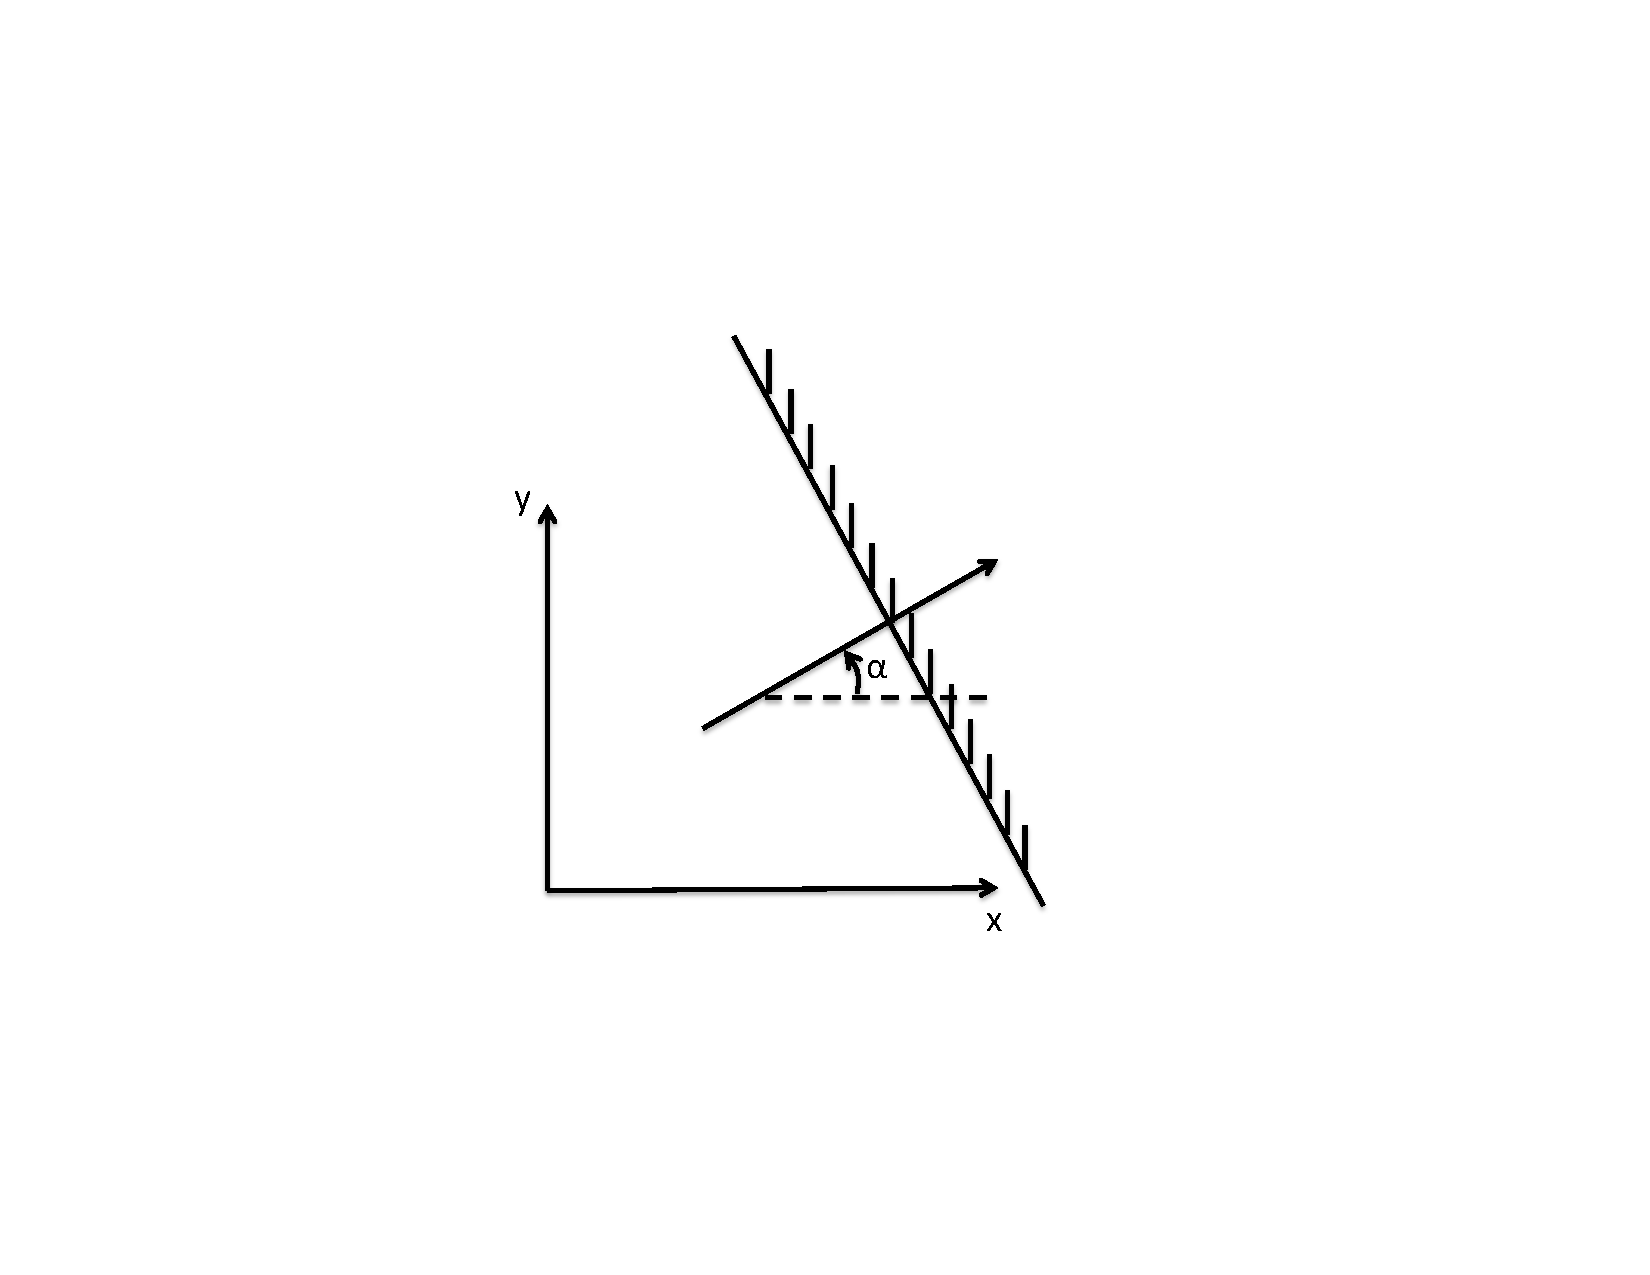
\includegraphics[width=0.6\textwidth]{../figures/beach_direction.pdf}
	\caption{Definition of an angle between $x-$axis and beach-normal direction.}
	\label{beach_angle}
\end{figure}


The bedload transport rates can be expressed as
\be
q_{bc} = \frac{b P_b}{g (s-1)} \sigma^3_T (1+ U_* V_*^2 +2 F_m \sin \theta) G_s
\ee 
\be
q_{bl} = \frac{b P_b}{g (s-1)} \sigma^3_T \left[ V_* (1+U^2_* + V^2_*) -2 r_m \sin \theta  \right ]
\ee
where $b$ is empirical bedload parameter; $\sigma_T$ is standard deviation of the oscillatory depth-averaged velocity with zero mean;  $(U_*, V_*) = (\bar{U}_c/\sigma_T, \bar{V}_l/\sigma_T)$;     $\theta$ is wave angle; and 
\be
r_m = -(U_*\cos \theta + V_* \sin \theta)
\ee
\be
F_m = V_* \cos \theta - U_* \sin \theta
\ee
$G_s$ is the bottom slope function expressed by
\ba
\left \{ \begin{array}{l l l}
G_s = \tan \phi /(\tan \phi + S_b)  &  \mbox{for}  &  -\tan \phi < S_b < 0 \\
G_s = (\tan \phi -2 S_b) /(\tan \phi -S_b)  & \mbox{for} & 0 < S_b < \tan \phi
\end{array} \right.
\ea
in which $\phi$ is the angle of internal friction of the sediment and $\tan \phi \simeq 0.63$ for sand.
  
In a general Cartesian system, ($q_{bc}, q_{bl}$) are converted to ($q_{bx}, q_{bl}$) using
\be
q_{bx} = q_{bc} \cos \alpha - q_{bl} \sin \alpha,  \ \ \ \ \ \  q_{by} = q_{bc} \sin \alpha + q_{bl} \cos \alpha
\ee

\subsection{Seabed evolution equation}

        The sea bed evolution equation can be described using sediment transport flux in generalized curvilinear coordinates:
\be  
 (1-p) \frac{\partial h}{\partial t} + \frac{1}{J} \frac{\partial J f_{mor} q_\beta L^\alpha_\beta}{\partial \xi^\alpha} = 0
  \label{bed}
\ee
where $p$ is the bed porosity,  $f_{mor}$ represents a morphology factor. (\ref{bed}) is solved using the same TVD scheme as in SHORECIRC.  

\section{Numerical schemes for SHORECIRC}

\subsection{Compact form of governing equations}

The compact form of governing equations can be written as
\be
\frac{\partial {\bf \Psi}}{\partial t} + \nabla \cdot {\bf \Theta}({\bf \Psi}) = {\bf S}
\label{tvd}
\ee
where ${\bf \Psi}$ and ${\bf \Theta} ({\bf \Psi})$ are  the vector of conserved variables and  the flux vector function, respectively, and are given by
\ba
{\bf \Psi} = \left( \begin{array}{c} J\eta \\
JP \\
JQ \end{array} \right) 
\ea
\ba
 {\bf \Theta} = \left( \begin{array}{c}
JP {\bf i} + JQ {\bf j} \\
\left[JPu +\frac{1}{2}g (\eta^2 + 2 \eta h)JL^1_1 \right ] {\bf i} + \left[JQu +\frac{1}{2}g (\eta^2 + 2 \eta h)JL^2_1 \right ] {\bf j} \\
\left[JPv +\frac{1}{2}g (\eta^2 + 2 \eta h)JL^1_2 \right ]  {\bf i} + \left[JQv +\frac{1}{2}g (\eta^2 + 2 \eta h)JL^2_2 \right ] {\bf j} 
\end{array}
\right) .
\ea

\ba
{\bf S} = \left( \begin{array}{c} 
0\\
\frac{1}{\rho} \left(F_{\mbox{wx}}  -\tau^b_x + \tau^s_x -f_x,  - ROT_x \right) \\
\frac{1}{\rho} \left(F_{\mbox{wy}}  -\tau^b_y + \tau^s_y  -f_y - ROT_y \right) 
\end{array}
\right) ,
\ea
where $(u,v)$ represent Cartesian components of velocity, $(P,Q) = (Hu^1, Hu^2)$, the contravariant components of flow flux,  ($\tau^b_x, \tau^b_y$),  ($\tau^b_x, \tau^b_y$), ($f_x, f_y$) and ($ROT_x, ROT_y$) represent the bottom friction, wind stress,  Coriolis forcing and the rest of terms in $x$ and $y$ directions, respectively. 
($F_{\mbox{wx}},  F_{\mbox{wy}}$) are the gradient of radiation stresses expressed by
\be
F_{\mbox{wx}} = -  \left [ \frac{\partial }{\partial \xi^1} \left (S_{xx} J L^1_1+S_{xy} J L^1_2 \right) + 
 [ \frac{\partial }{\partial \xi^2} \left (S_{xx} J L^2_1+S_{xy} J L^2_2 \right)
 \right ]
\ee 
\be
F_{\mbox{wy}} = -  \left [ \frac{\partial }{\partial \xi^1} \left (S_{xy} J L^1_1+S_{yy} J L^1_2 \right) + 
 [ \frac{\partial }{\partial \xi^2} \left (S_{xy} J L^2_1+S_{yy} J L^2_2 \right)
 \right ]
\ee 
The reason to put the wave forcing as a source term rather than a flux term is that the forcing  is calculated directly from SWAN in a curvilinear grid. 



\subsection{Spatial discretization}

A combined finite-volume and finite-difference method was applied to the spatial discretization. For the flux terms and the first-order derivative terms, 
 MUSCL-TVD schemes from the 2nd-order to 4th-order  are implemented in the present model. The multi-order MUSCL-TVD scheme can be written in a compact form  according to Erduran et al. (2005) who modified Yamamoto et al.'s (1995)  fourth-order approach. 
In $x$-direction, for example, the combined form of the interface construction can be written as follows:
\be
\phi^L_{i+1/2} = \phi_i +\frac{1}{4} \left[ (1-\kappa_1)\chi(r) \Delta^* \phi_{i-1/2} + (1+\kappa_1) \chi(1/r) \Delta^* \phi_{i+1/2} \right ]
\label{left}
\ee
\be
\phi^R_{i-1/2} = \phi_i -\frac{1}{4} \left[ (1+\kappa_1)\chi(r) \Delta^* \phi_{i-1/2} + (1-\kappa_1) \chi(1/r) \Delta^* \phi_{i+1/2} \right ]
\label{right}
\ee
where $\phi^L_{i+1/2} $ is the constructed value at the left-hand side of the interface $i+\frac{1}{2}$ and  $\phi^R_{i-1/2} $ is the value at the right-hand side of the interface $i - \frac{1}{2}$.  The values of $\Delta^* \phi$ are evaluated as follows:
\ba
\nonumber
&&\Delta^* \phi_{i+1/2} = \Delta \phi_{i+1/2} - \kappa_2 \Delta^3 \bar{\phi}_{i+1/2} /6, \\
\nonumber && \Delta \phi_{i+1/2} = \phi_{i+1} - \phi_{i} ,\\
\nonumber  && \Delta^3 \bar{\phi}_{i+1/2} = \Delta \bar{\phi}_{i+3/2} - 2 \Delta \bar{\phi}_{i+1/2} + \Delta \bar{\phi}_{i-1/2}, \\
\nonumber && \Delta \bar{\phi}_{i-1/2} =\mbox{minmod} (\Delta \phi_{i-1/2}, \Delta \phi_{i+1/2}, \Delta \phi_{i+3/2}) , \\
\nonumber &&  \Delta \bar{\phi}_{i+1/2} =\mbox{minmod} (\Delta \phi_{i+1/2}, \Delta \phi_{i+3/2}, \Delta \phi_{i-1/2}) , \\
\nonumber && \Delta \bar{\phi}_{i+3/2} =\mbox{minmod} (\Delta \phi_{i+3/2}, \Delta \phi_{i-1/2}, \Delta \phi_{i+1/2}) \\
\label{minmod}
\ea 
In (\ref{minmod}), minmod represents the minmod limiter and is given by
\be
\mbox{minmod} (j,k,l) = \mbox{sign} (j) \mbox{max} \{ 0, \mbox{min} [|j|, 2 \mbox{sign} (j) k, 2 \mbox{sign} (j) l ] \} .
\ee
$\kappa_1$ and $\kappa_2$ in (\ref{left}) and (\ref{right}) are  control parameters for orders of the scheme in the compact form.  The complete form with $(\kappa_1, \kappa_2) = (1/3, 1)$ is the fourth-order scheme given by Yamamoto et al. (1995). $(\kappa_1, \kappa_2) = (1/3, 0)$ yields a third-order scheme, while the second-order scheme can be retrieved using  $(\kappa_1, \kappa_2) = (-1, 0)$. 

$\chi(r)$ in (\ref{left}) and (\ref{right}) is the limiter function. The original scheme introduced by Yamamoto et al. (1998) uses the Minmod limiter as used in (\ref{minmod}). Erduran et al. (2005) found that the use of the van-Leer limiter for the third-order scheme gives more accurate results. Their finding was confirmed by  using the present model in the benchmark tests for wave runup conducted by Tehranirad et al. (2011).  The van-Leer limiter can be expressed as
\be
\chi(r) = \frac{r+|r|}{1+r}
\ee
where
\be
r = \frac{\Delta^* \phi_{i+1/2}}{\Delta ^* \phi_{i-1/2}}.
\ee

The numerical fluxes are computed using a HLL approximate Riemann solver

\be
{\bf \Theta} ({\bf \Psi}^L, {\bf \Psi}^R)= \left \{ \begin{array}{ll} {\bf \Theta} ({\bf \Psi}^L) & \mbox{if} \ \ \ s_L \ge 0 \\
{\bf \Theta}^* ({\bf \Psi}^L, {\bf \Psi}^R) & \mbox{if} \ \ \ s_L < 0 < s_R \\
{\bf \Theta}({\bf \Psi}^R) & \mbox{if} \ \ \ s_R \le 0,
\end{array}  \right.
\ee
where
\be
{\bf \Theta^*} ({\bf \Psi}^L, {\bf \Psi}^R) = \frac{s_R {\bf \Theta} ({\bf \Psi}^L) -s_L {\bf \Theta}({\bf \Psi}^R) + s_L s_R ({\bf \Psi}^R - {\bf \Psi}^L)}{s_R - s_L}
\ee
The wave speeds of the Riemann solver are given by
\be
s_L= \mbox{min} ({\bf V}^L \cdot {\bf n} - \sqrt{g (h+\eta)^L} , u_s -\sqrt{\varphi_s}),  
\label{sl}
\ee
\be
s_R= \mbox{max} ({\bf V}^R \cdot {\bf n} + \sqrt{g (h+\eta)^R},  u_s +\sqrt{\varphi_s}),  
\label{sr}
\ee
in which $u_s$ and $\varphi_s$ are estimated as
\be
u_s =\frac{1}{2} ({\bf V}^L + {\bf V}^R)\cdot {\bf n} + \sqrt{g (\eta + h)^L} - \sqrt{g(\eta+h)^R}
\ee
\be
\sqrt{\varphi_s} = \frac{\sqrt{g (\eta + h)^L}+\sqrt{g (\eta + h)^R}}{2} +\frac{({\bf V}^L - {\bf V}^R)\cdot {\bf n}}{4}
\ee
and ${\bf n}$ is the normalized side vector for a cell face.


\subsection{Time stepping}

The third-order Strong Stability-Preserving (SSP) Runge-Kutta scheme for nonlinear spatial discretization (Gottlieb et al., 2001) was adopted for time stepping. The scheme is given by
\ba
\nonumber
&& {\bf \Psi}^{(1)} = {\bf \Psi}^{n}  + \Delta t (- \nabla \cdot {\bf \Theta} ({\bf \Psi}^n) + {\bf S}^{(1)} ) \\
&&  {\bf \Psi}^{(2)} = \frac{3}{4}{\bf \Psi}^{n}  + \frac{1}{4} \left[   {\bf \Psi}^{(1)} +  \Delta t \left (- \nabla \cdot {\bf \Theta} ({\bf \Psi}^{(1)} ) + {\bf S}^{(2)} \right) \right] \\
\nonumber
&&  {\bf \Psi}^{n+1} = \frac{1}{3}{\bf \Psi}^{n}  + \frac{2}{3} \left[   {\bf \Psi}^{(2)} +  \Delta t \left (- \nabla \cdot {\bf \Theta} ({\bf \Psi}^{(2)} ) + {\bf S}^{n+1} \right) \right]
\label{runge}
\ea
in which ${\bf \Psi}^{n}$ denotes ${\bf \Psi}$  at time level $n$.  ${\bf \Psi}^{(1)}$ and ${\bf \Psi}^{(2)}$ are values at intermediate stages in the Runge-Kutta integration. 

An  adaptive time step is chosen, following the Courant-Friedrichs-Lewy (CFL) criterion:
\be
\Delta t = C  \mbox{min} \left ( \mbox{min} \frac{\Delta x}{|u_{i,j}| + \sqrt{g (h_{i,j} +\eta_{i,j})}},  \mbox{min} \frac{\Delta y}{|v_{i,j}| + \sqrt{g (h_{i,j} +\eta_{i,j})}} \right )
\label{cfl}
\ee
where $C$ is the Courant number and $C=0.5$ was used in the following examples.  

\subsection{Wetting-drying schemes for shallow water}

The wetting-drying scheme for modeling  a moving boundary is straightforward. The normal flux ${\bf n} \cdot {\bf M}$ at the cell interface of a dry cell is set to zero. A mirror boundary condition is applied to the high-order MUSCL-TVD scheme. It may be noted that the wave speeds of the Riemann solver  (\ref{sl}) and (\ref{sr}) for a dry cell are modified as 
\be
s_L= {\bf V}^L \cdot {\bf n} - \sqrt{g (h+\eta)^L} ,  \ \ \ \    s_R= {\bf V}^L \cdot {\bf n} +2  \sqrt{g (h+\eta)^L}  \  \  \  \mbox{(right dry cell)}
\ee
and
\be
s_L= {\bf V}^R \cdot {\bf n} - \sqrt{g (h+\eta)^R} ,  \ \ \ \    s_R= {\bf V}^R \cdot {\bf n} +2  \sqrt{g (h+\eta)^R}  \  \  \  \mbox{(left dry cell)}
\ee


\subsection{Boundary conditions}

To incorporate tide and river inflow into the circulation module, two types of open boundary conditions are implemented. One is the surface clamped boundary condition that reads
                                                      at tidal open boundaries                          
\be
\eta= \eta_0    \ \ \ \ \ \ \mbox{at tidal open boundaries}
\ee                                                      
where  $\eta_0$ is measured or predicted surface elevations at open boundaries. The other is the specified flux boundary condition that is usually used at river boundaries:
\be
P^\alpha = Q^{\mbox{flux}}_\beta L^\alpha_\beta
\ee                                                                                                         
where  $Q^{\mbox{flux}}$ is the specified volume flux per unit width. 


\section{SWAN-SHORECIRC coupling and parallelization}

For the SHORECIRC code,  we used a domain decomposition technique to subdivide the problem into multiple regions and assign each subdomain to a separate processor core. Each 
subdomain region contains an overlapping area of ghost cells,  three-row deep, as required by the highest-order ( the fourth order) MUSCL-TVD scheme in the model. The Message Passing Interface (MPI) with non-blocking communication is used to exchange  data in the overlapping region between neighboring processors. 

For the SWAN code, we used the existing domain decomposition scheme which is slightly different from the SHORECIRC code. The version  40.51AB of SWAN uses a single-direction domain decomposition and takes into account number of dry points in the grid splitting. Because of the different domain decomposition between SHORECIRC and SWAN, it  is difficult to directly pass variables between the decomposed domains. We now used a two-step mapping method which is  to first gather a passing variable into the global domain, and then to distribute it into each sub-domain. Dry points in SWAN are set to be wet with a small water depth (1 mm) in order to make an equal split of a computational domain. 

Figure \ref{domain} shows an example of domain decomposition in SWAN and SHORECIRC. 

To investigate performance of the parallel program, numerical simulations of an 
idealized  case are tested with different numbers of processors  on a Linux cluster located at University of Delaware. 
The test case is set up in a numerical grid  of 1800 $\times$ 1800 cells.  
Figure \ref{fig1} shows the model speedup versus number of processors. It can be seen that performance scales nearly proportional to the number of processors, with some delay caused by inefficiencies in parallelization, such as inter-processor communication time.


\begin{figure}[htbp]
\centering
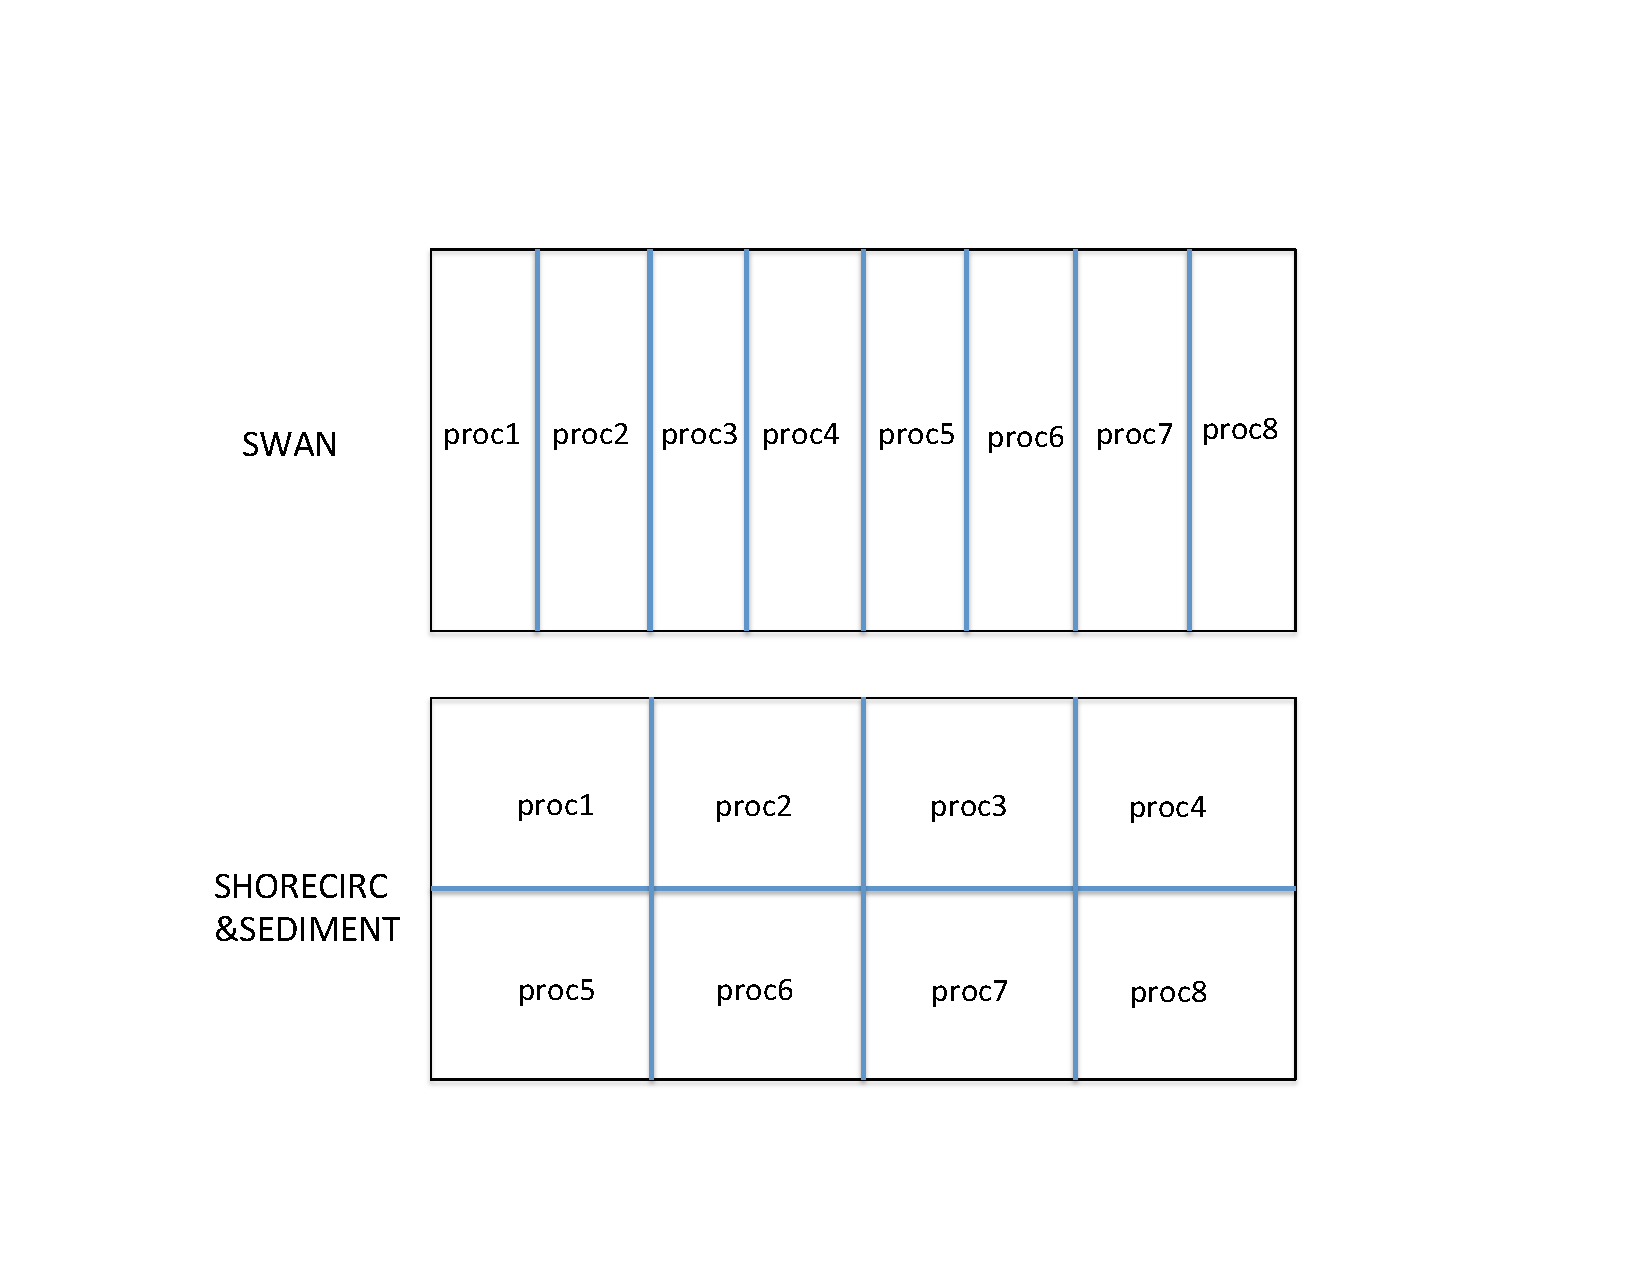
\includegraphics[width=1.0\textwidth]{../figures/parallel.pdf}
\caption{An example of domain decomposition in SWAN and SHORECIRC/SEDIMENT.}
\label{domain}
\end{figure}

\begin{figure}[htbp]
\centering
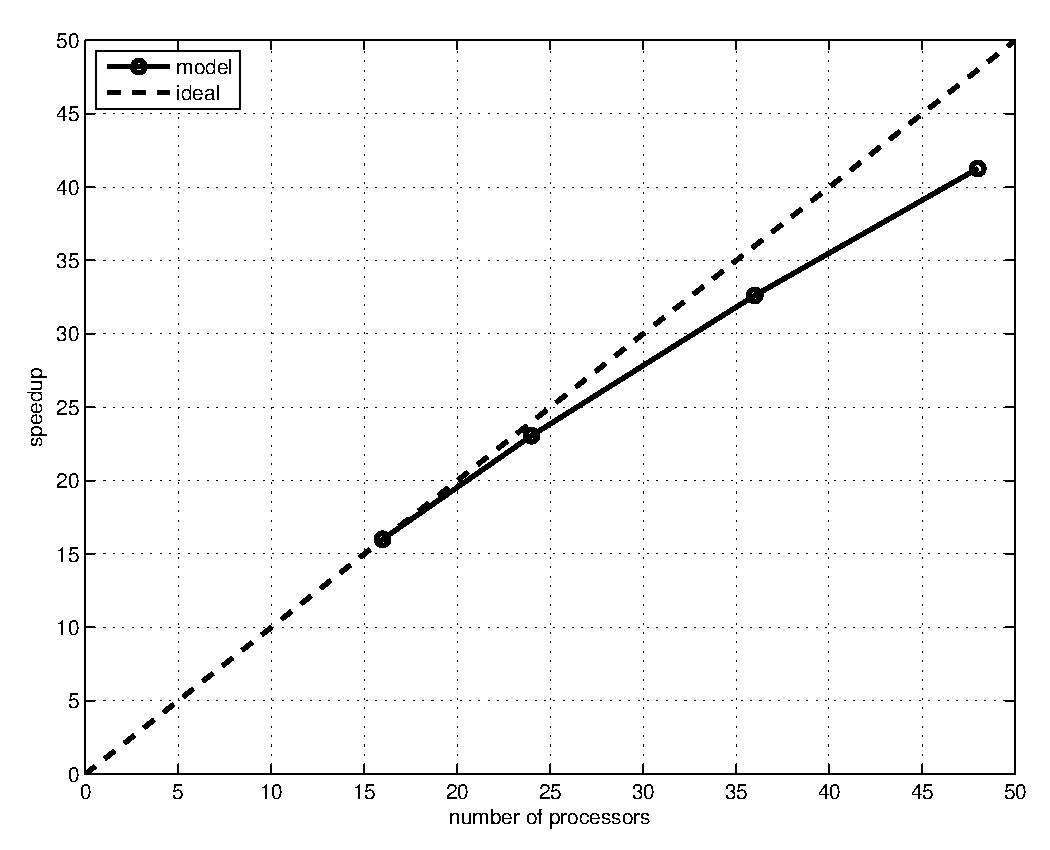
\includegraphics[width=0.8\textwidth]{../figures/speedup.eps}
\caption{Variation in model performance with number of processors for a 1800 x 1800 domain.  Straight line indicates arithmetic speedup. Actual performance is shown in the curved line ({\bf the figure needs to be updated using the coupled model !!!}).}
\label{fig1}
\end{figure}


\newpage

\section{Users' Manual}

\subsection{Program outline and flow chart}

The code was written using Fortran 90 with the c preprocessor (cpp) statements for separation of the source code. Arrays are dynamically allocated at runtime. Precision is selected using the {\em selected\_real\_kind} Fortran intrinsic function defined in the makefile.  The default precision is single. 

The present version of NearCoM-TVD includes a number of options including (1) choice of serial or parallel code (2) Cartesian or curvilinear coordinate, (3) samples.

The flow chart is shown in Figure {\ref{chart}}. 

\begin{figure}[htbp]
	\centering
		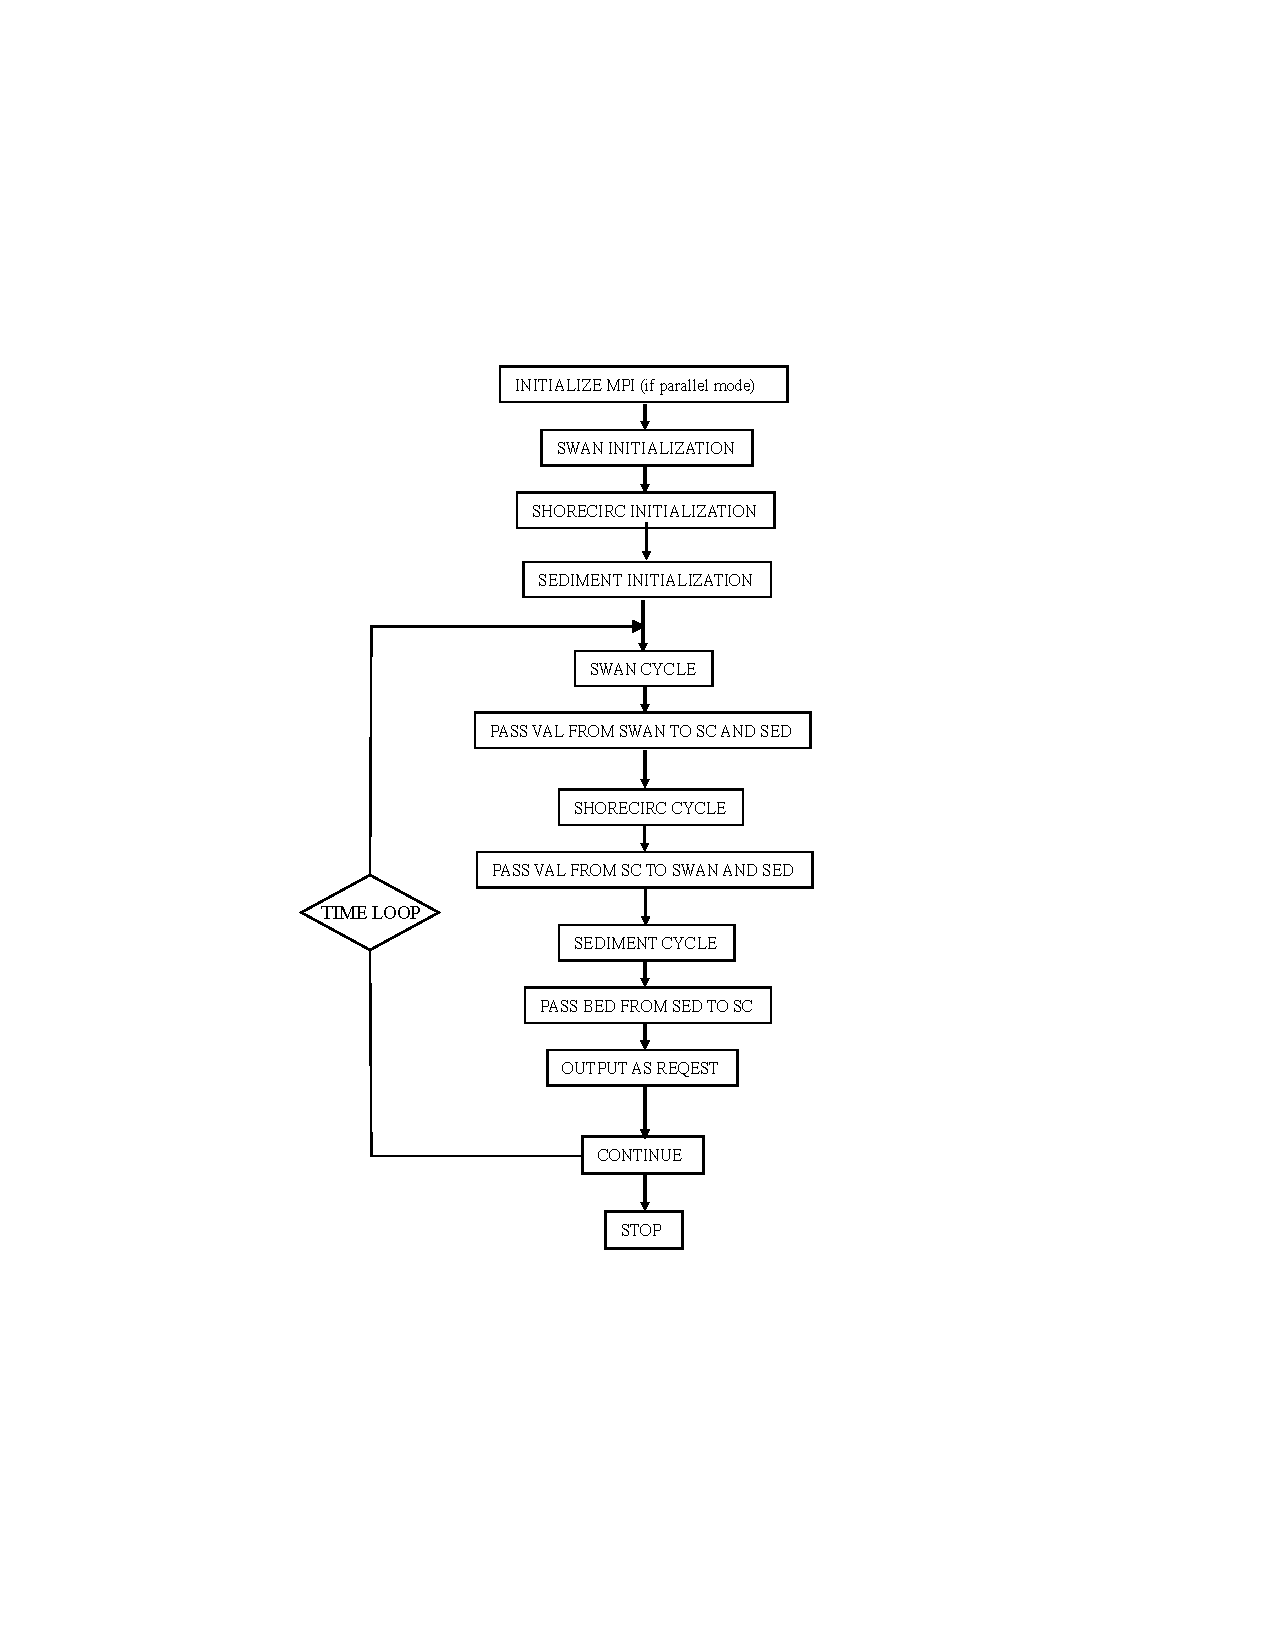
\includegraphics[width=0.8\textwidth]{../figures/CHART.pdf}
	\caption{Flow chart of the main program.}
	\label{chart}
\end{figure}

\subsection{Permanent variables associated with coupling}

\begin{description}

\item  Depth(): still water depth $h$ at element point
\item  DepthX(): still water depth $h$ at x-interface
\item  DepthY(): still water depth $h$ at y-interface
\item  Eta():   surface elevation, for dry point, Eta() = MinDepth - Depth(), MinDepth is specified in input.txt. 
\item  Eta0(): $\eta$ at previous time level

\item  MASK(): 1 - wet,       0 - dry
\item  MASK\_STRUC(): 0 - permanent dry point

\item  U():  depth-averaged $u$ 
\item  V():  depth-averaged $v$ 

\item  Uc():  contravariant component of depth-averaged velocity in $\xi_1$ direction 
\item  Vc(): contravariant component of depth-averaged velocity in $\xi_2$ direction 

\item  HU(): $(h+\eta)  u$ at element
\item  HV(): $(h+\eta)  v$ at element
\item  P(): $(h+\eta) U $ at x-interface for Cartesian, and $(h+\eta) Uc $ at $\xi_1$-interface curvilinear
\item  Q(): $(h+\eta) V $ at y-interface for Cartesian, and $(h+\eta) Vc $ at $\xi_2$-interface curvilinear
\item  Fx(): numerical flux F at x-interface
\item  Fy(): numerical flux F at y-interface
\item  Gx(): numerical flux G at x-interface
\item  Gy(): numerical flux G at y-interface
\item  Ubar(): $HU$ for Cartesian and  $JHU$ for curvilinear
\item  Vbar(): $HV$ for Cartesian and $JHV$ for curvilinear


\item  EtaRxL(): $\eta$ Left value at x-interface
\item  EtaRxR(): $\eta$ Right value at x-interface
\item  EtaRyL(): $\eta$ Left value at y-interface
\item  EtaRyR(): $\eta$ Right value at y-interface
\item  HxL():   total depth  Left value at x-interface
\item  HxR():   total depth  Right value at x-interface
\item  HyL():   total depth  Left value at y-interface
\item  HyR():   total depth  Right value at y-interface

\item  HUxL(): $(h+\eta)u$ Left value at x-interface
\item  HUxR(): $(h+\eta)u$ Right value at x-interface
\item  HVyL(): $(h+\eta)v$ Left value at y-interface
\item  HVyR(): $(h+\eta)v$ Right value at y-interface

\item  PL(): Left P  value at x-interface
\item  PR(): Right P value at x-interface
\item  QL():  Left  Q value at y-interface
\item  QR(): Right Q value at y-interface

\end{description}


\subsection{Installation and compilation}

NearCoM-TVD is distributed in a compressed fie. To install the programs, first, uncompress the package. Then use 

$>$ tar xvf *.tar 

\noindent
to extract files from the uncompressed package. The exacted files will be distributed in two new directories: /CIRC\_SWAN and /work.

To compile the program, go to /CIRC\_SWAN and modify Makefile if needed. There are several necessary flags in Makefile needed to specify below.

\begin{description} 

\item -DDOUBLE\_PRECISION: use double precision, default is single precision.

\item -DPARALLEL: use parallel mode, default is serial mode.

\item -DSAMPLES: include all samples, default is no sample included.

\item -DCURVILINEAR: curvilinear version, otherwise Cartesian.  \\ {\bf NOTE:} setting curvilinear is a must for SWAN and SHORECIRC coupled model.

\item -DSEDIMENT: include sediment and seabed modules.

\item -DINTEL: INTEL compiler.

\item -DRESIDUAL: include tidal residual calculation.

\item -DSTATIONARY: stationary mode for SHORECIRC

\item CPP: path to CPP directory.

\item FC: Fortran compiler. 

\end{description}
Then execute 

$>$ make clean

$>$ make

\noindent
The executable file `'nearcom' will be generated and  copied from /CIRC\_SWAN to /work/. Note: use `make clean' after any modification of  Makefile.  

To run the model, go to /work. Modify INPUT if needed and run. 


\subsection{Input}

Following are descriptions of parameters in input.txt
({\bf  NOTE: }  all parameter names are capital sensitive).

 \begin{description}
 
\item {\bf SWAN INPUT:}   refer to SWAN manual. Model run time is set in SWAN model. For example,

COMPUTE NONSTAT 20081114.160000 1 MI 20081114.230000 

The above setting means model run start from 2008 11 14 16:00 to 2008 11 14 23:00. The model call swan at  $DT_{\mbox{swan}}$ = 1 minute. The loop number for SHORECIRC and SEDIMENT is estimated by  $DT_{\mbox{swan}}$ and the time step of SHORECIRC (time varying).

{\bf IMPORTANT SETTING IN SWAN:}

    1) in SET, always set CARTESIAN in order to make a grid orientation consistent with SHORECIRC
    
    2) in SET, always set [inrhog] as 1 to get a true wave energy dissipation.
    
    3)in COMPUTE, always set NONSTAT mode. 

\item {\bf WAVE CURRENT INTERACTION}

\item SWAN\_RUN: logical parameter to run SWAN

\item SHORECIRC\_RUN: logical parameter to run SHORECIRC 

\item WC\_BOUND\_WEST:  west bound region  (number of grid point) in which  wave-current is inactive. 

\item WC\_BOUND\_EAST : east bound region  (number of grid point) in which  wave-current is inactive.

\item WC\_BOUND\_SOUTH : south bound region  (number of grid point) in which  wave-current is inactive.

\item WC\_BOUND\_NORTH: north bound region  (number of grid point) in which  wave-current is inactive.

\item WC\_LAG :  time delay for wave-current interaction

\item {\bf TITLE}: title for SHORECIRC log file
      
\item {\bf SPECIFICATION OF MULTI-PROCESSORS}

\item PX:  processor numbers in X
\item PY :  processor numbers in Y \\
 {\bf NOTE:} PX and PY must be consistency with number of processors defined in mpirun command, e.g., 
mpirun -np n (where n = px$\times$py). 

 
 \item {\bf SPECIFICATION OF WATER DEPTH}
 
 \item DEPTH\_TYPE: depth input type. 
 
   DEPTH\_TYPE=DATA: from a depth file. 
   
   The program includes several simple bathymetry configurations such as
   
                DEPTH\_TYPE=FLAT:  flat bottom, need DEPTH\_FLAT 
                
                DEPTH\_TYPE=SLOPE:  plane beach along $x$ direction. It needs three parameters:
                                    slope,SLP,  slope starting point, Xslp
                                   and flat part of depth, DEPTH\_FLAT

\item  DEPTH\_FILE: bathymetry file if  DEPTH\_TYPE=DATA, file dimension should be Mglob x Nglob with the first point as the south-west corner.  The read format in the code is shown below.

       DO J=1,Nglob
       
        READ(1,*)(Depth(I,J),I=1,Mglob)
        
       ENDDO
 
\item DEPTH\_FLAT: water depth of flat bottom if DEPTH\_TYPE=FLAT or DEPTH\_TYPE=SLOPE (flat part of a plane beach).
 
\item SLP: slope if DEPTH\_TYPE=SLOPE

\item Xslp: starting $x$ (m) of a slope, if DEPTH\_TYPE=SLOPE


 \item {\bf SPECIFICATION OF RESULT FOLDER}  
  
\item RESULT\_FOLDER: result folder name, e.g., RESULT\_FOLDER = /Users/fengyanshi/tmp/

 \item {\bf SPECIFICATION OF DIMENSION}

\item Mglob: global dimension in $x$ direction.

\item Nglob: global dimension in $y$ direction. \\
{\bf NOTE:} For parallel runs, Mglob and Nglob can be divided by PX and PY, respectively. MAX(Mglob,Nglob) can be divided by PX $\times$ PY.

\item {\bf SPECIFICATION OF STATIONARY MODE}

\item N\_ITERATION: the iteration number for stationary mode of SHORECIRC (set -DSTATIONARY in Makefile).

\item WATER\_LEVEL\_FILE:  the file name of water level file containing time and water level, for stationary mode. The following example shows the format. 

water levels for stationary mode \\
5   - number of water level data\\
0.0       0.0 ! Time (s), Level (m) \\
3600.0    0.5  \\
7200.0    0.8660 \\
10800.0   1.0  \\
14400.0   0.866  \\
18000.0   0.5 \\

 \item {\bf SPECIFICATION OF TIME}
 
\item PLOT\_INTV: output interval in seconds (Note, output time is not exact because adaptive dt is used.)

\item SCREEN\_INTV: time interval (s) of screen print. 

\item PLOT\_INTV\_STATION: time interval (s) of gauge output

 \item {\bf SPECIFICATION OF GRID}

\item DX: grid size(m) in $x$ direction, for Cartesian mode

\item DY:   grid size(m) in $y$ direction, for Cartesian mode

\item X\_FILE: name of file to store x for curvilinear mode

\item Y\_FILE: name of file to store y for curvilinear mode

{\bf NOTE:} data format is the same as the depth data shown above. 

\item CORI\_CONSTANT: logical parameter for constant Coriolis parameter

\item LATITUDE: latitude if constant Coriolis parameter is used

\item LATITUDE\_FILE: name of file to store latitude at every grid point if not constant Coriolis

{\bf NOTE:} data format is the same as the depth data shown above. 

\item {\bf BOUNDARY CONDITIONS}

\item ETA\_CLAMPED: logical parameter for surface elevation clamped condition  

\item V\_CLAMPED: logical parameter for velocity clamped condition  

\item FLUX\_CLAMPED: logical parameter for flux clamped condition  

\item TIDE\_FILE: name of file to store tidal constituents 

{\bf DATA FORMAT:}  please refer to mk\_tide.f90. 
The formula of surface elevation at a tidal boundary can be expressed by
\be
\eta_0 (t) =  \sum_{n=1}^Na_{0}({\bf x}, n) f_c (n) \cos \left(\frac{2\pi}{T(n)} t - \phi({\bf x}, n)  + (V_0 +u_0)(n) \right)
\ee 
where $a_0$  and $\phi$ represent amplitude and phase lag, respectively, for a harmonic constituent at location $\bf x$. $T$ is tidal period. $f_c$ and $(V_0+u_0)$ are the lunar node factor and the equilibrium argument, respectively,  for a constituent. 

The following is an example of M2 + O1.

tidal boundary conditions \\
 150 --- number of days from Jan 1,  to simulation date \\ 
  2 ---  number of constituents \\
       1.000       0.000   --- $f_c$ and $(V_0+u_0)$ for M2\\
       0.980       0.000  ---   $f_c$ and $(V_0+u_0)$ for O1\\
          80   ---  number of tidal boundary points \\
    1 ,   1   ---  (i,j) grid location of tidal boundary  \\\
      12.420       1.200       21.000   --- $T$, amplitude $a_0$ and phase lag $\phi$ for M2 \\
       24.000       0.3          30.100   -- $T$, amplitude $a_0$ and phase lag $\phi$ for O1 \\
    2 ,   1   ---  (i,j) grid location of tidal boundary  \\\
      12.420       1.200       21.000   --- $T$, amplitude $a_0$ and phase lag $\phi$ for M2 \\
       24.000       0.3          30.100   -- $T$, amplitude $a_0$ and phase lag $\phi$ for O1 \\
    3 ,  1 \\
    ...
   

\item FLUX\_FILE: name of file to store time series of flux (e.g., unit width river flux) 


{\bf DATA FORMAT:} \\
title\\
Number of data, Number of flux point \\
I, J, River orientation \\
Time, Flux, Angle in Cartesian \\
...  \\
where  (I,J) represent grid points of river location. River orientation represents the direction which a river flows from  in the  IMAGE domain (for curvilinear coordinates).  
Use W,E,S and N for the orientation.  For example, `W' represents a river flowing into the domain from the west boundary (in IMAGE domain for curvilinear coordinates).

Please refer to mk\_river.f90. The following is an example.

 river flux boundary condition \\
       5       2     ! NumTimeData, NumFluxPoint \\
   1  38  W      ! I, J, River\_Orientation\\
       0.000       0.200       0.000\\
  360000.000       0.200       0.000\\
  720000.000       0.200       0.000\\
 1080000.000       0.200       0.000\\
 1440000.000       0.200       0.000\\
   1  39  W      ! I, J, River\_Orientation\\
       0.000       0.200       0.000\\
  360000.000       0.200       0.000\\
  720000.000       0.200       0.000\\
 1080000.000       0.200       0.000\\
 1440000.000       0.200       0.000\\
 end of file\\


\item{\bf WIND CONDITION}

Spatially uniform wind field is assumed in this version.  

\item WindForce: logical parameter for wind condition, T or F. 

\item WIND\_FILE: name of file for a time series of wind speed.

{\bf DATA FORMAT:} the following is an example of wind data.

wind data

100  - number of data

0.0 ,    -10.0 0.0   ---  time(s), wu, wv (m/s)

2000.0,   -10.0,  0.0

8000.0,  -10.0,   0.0
 
... 


\item Cdw: wind stress coefficient for the quadratic formula. 

 \item {\bf SPECIFICATION OF INITIAL CONDITION}
 
 \item INT\_UVZ : logical parameter for initial condition, default is FALSE
 
 
\item ETA\_FILE: name of file for initial $\eta $, e.g., ETA\_FILE= /Users/fengyanshi/work/input/CVV\_H.grd, data format is the same as depth data.

\item U\_FILE:  name of file for initial $u$, e.g.,U\_FILE= /Users/fengyanshi/work/input/CVV\_U.grd, data format is the same as depth data.

\item V\_FILE:  name of file for initial $v$, e.g., V\_FILE= /Users/fengyanshi/work/input/CVV\_V.grd, data format is the same as depth data.

 \item {\bf SPECIFICATION OF WAVEMAKER}
 
 There is no wavemaker implemented in SHORECIRC.

\item {\bf SPECIFICATION OF PERIODIC BOUNDARY CONDITION} 

( Note: only south-north periodic condition was implemented)

\item PERIODIC\_X: logical parameter for periodic boundary condition in x direction, T - periodic, F - wall boundary condition.

\item PERIODIC\_Y: logical parameter for periodic boundary condition in x direction.

\item Num\_Transit: grid numbers needed to make periodic condition for SWAN. The reason to set this parameter is that SWAN doesn't have an option for periodic boundary condition. In this implementation, a periodic boundary condition is implemented by making a transition from  a left array ( count to Num\_Transit from left boundary) to a right array. 

\item {\bf SPECIFICATION OF SPONGE LAYER} 
 
 \item SPONGE\_ON: logical parameter, T - sponge layer, F - no sponge layer.
 
\item Sponge\_west\_width: width (m) of sponge layer at west boundary.

\item Sponge\_east\_width:   width (m) of sponge layer at east boundary.

\item Sponge\_south\_width: width (m) of sponge layer at south boundary.

\item Sponge\_north\_width width (m) of sponge layer at north boundary

\item R\_sponge: decay rate in sponge layer. Its values are between 0.85 $\sim$ 0.95.

\item A\_sponge: maximum damping magnitude. The value is $\sim$ 5.0. 

\item {\bf SPECIFICATION OF OBSTACLES} 

\item OBSTACLE\_FILE: name of obstacle file. 1 - water point, 0 - permanent dry point. Data dimension is (Mglob $\times$ Nglob). Data format is the same as the depth data. 
 
 \item {\bf SPECIFICATION OF PHYSICS} 
  
\item Cd: quadratic bottom friction coefficient 

\item nu\_bkgd : background eddy viscosity parameter. 
  
\item {\bf SPECIFICATION OF NUMERICS} 

\item Time\_Scheme: stepping option,  Runge\_Kutta or Predictor\_Corrector (not suggested for this version).

\item HIGH\_ORDER: spatial scheme option,  FOURTH for the fourth-order, THIRD for the third-order, and SECOND for the second-order (not suggested for Boussinesq modeling).

\item CONSTRUCTION: construction method,  HLL for HLL scheme, otherwise for averaging scheme.

\item CFL: CFL number, CFL $\sim$ 0.5.

\item FroudeCap: cap for Froude number in velocity calculation for efficiency. The value could be 5 $\sim$ 10.0.

\item MinDepth: minimum water depth (m) for wetting and drying scheme. Suggestion: MinDepth = 0.001 for lab scale and 0.01 for field scale. 

\item MinDepthFrc: minimum water depth (m) to limit bottom friction value. Suggestion: MinDepthFrc = 0.01 for lab scale and 0.1 for field scale. 


\item {\bf SPECIFICATION OF TIDAL RESIDUAL}

\item T\_INTV\_mean: time-averaging interval for Eulerian mean current and elevation. Note: use -DRESIDUAL in Makefile to make this option active.

\item {\bf SPECIFICATION OF SEDIMENT CALCULATION}

Note: set -DSEDIMENT in Makefile to make sediment module active

\item T\_INTV\_sed: time interval to call sediment module

\item Factor\_Morpho: morphology factor.
\item D\_50 : $D_{50}$
\item D\_90 : $D_{90}$
\item por:  sediment porosity
\item RHO: water density
\item nu\_water: water eddy viscosity
\item S\_sed: specific gravity
\item SOULSBY: logical parameter for Soulsby (1997) total load formula, T = true, F = false 
\item z0: $z_0$, bed roughness length. 
\item KOBAYASHI: logical parameter for KOBAYASHI's formula, T = true, F = false
\item angle\_x\_beach: coordinate rotation angle defined in Figure 1.
\item eB: $e_B$,  suspension efficiency for energy dissipation rate due to wave breaking
\item ef : $e_f$, suspension efficiency for energy dissipation rate due to bottom friction
\item a\_k: $a$, empirical suspended load parameter. 
\item b\_k : $b$, empirical bedload parameter.
\item TanPhi: $\tan \phi$, where $\phi$ is the angle of internal friction of the sediment. 
\item Gm: $G_m$ for slope function ($G_m=10$).
\item frc: friction coefficient in Kobayashi.
\item Si\_c: a coefficient in calculating $P_b$.


\item {\bf SPECIFICATION OF OUTPUT VARIABLES}

\item NumberStations: number of station for output. If NumberStations $> 0$, need input i,j in STATION\_FILE
 
\item DEPTH\_OUT: logical parameter for output depth. T or F. 
\item U: logical parameter for output $u$. T or F. 
\item  V: logical parameter for output $v$. T or F. 
\item ETA: logical parameter for output $\eta$. T or F. 
\item HS: logical parameter for output of significant wave height $H_s$. T or F. 
\item WFC: logical parameter for output of wave force. T or F. 
\item WDIR: logical parameter for output of peak wave direction. T or F. 
\item WBV: logical parameter for output of wave orbital velocity. T or F. 
\item MASK: logical parameter for output wetting-drying MASK. T or F. 
\item SourceX: logical parameter for output source terms in $x$ direction. T or F. 
\item SourceY:  logical parameter for output source terms in $y$ direction. T or F. 
\item UV3D: logical parameter for output 3D structure. T or F.
\item Qstk:   logical parameter for output Stokes mass flux. T or F.
\item DepDt:  logical parameter for output depth variation rate. T or F.
\item Qsed:  logical parameter for output sediment transport rate. T or F.

\end{description}
 

\subsection{Output}
The output files are saved in the result directory defined by RESULT\_FOLDER in INPUT. For outputs in ASCII,  a file name is a combination of variable name and an output series number such eta\_0001, eta\_0002, .... The format  and read/write algorithm are  consistent with a depth file.  Output for stations is a series of numbered files such as sta\_0001, sta\_0002 .... 

\section{Examples}

\subsection{An idealized case}

An idealized case is carried out to demonstrate a model run under several most useful conditions, including tide, wave, and river conditions. Figure \ref{depth} shows an idealized bathymetry which is constructed by a plane slope from a depth of 10 m to -1 m (dry points) and a channel with a depth of 2m located at the center of the beach.  A wave spectrum is specified at the south boundary. A tidal boundary condition (M2) is applied to the south boundary. River flux is provided at the inlet. The vertical wall boundary condition is applied to the west and east boundaries. 


\begin{figure}[htbp]
	\centering
		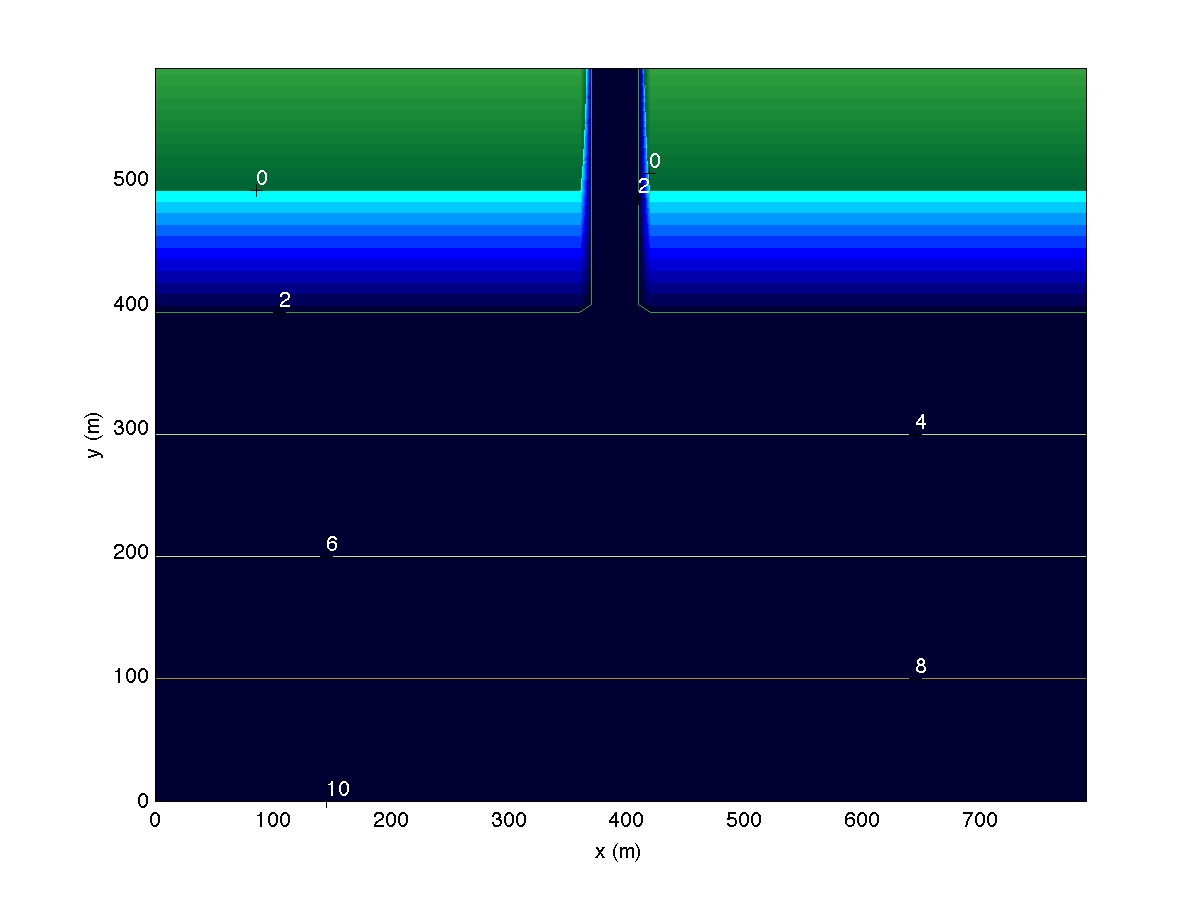
\includegraphics[width=0.8\textwidth]{../figures/ideal_depth.jpg}
	\caption{Idealized bathymetry.}
	\label{depth}
\end{figure}

\begin{figure}[htbp]
	\centering
		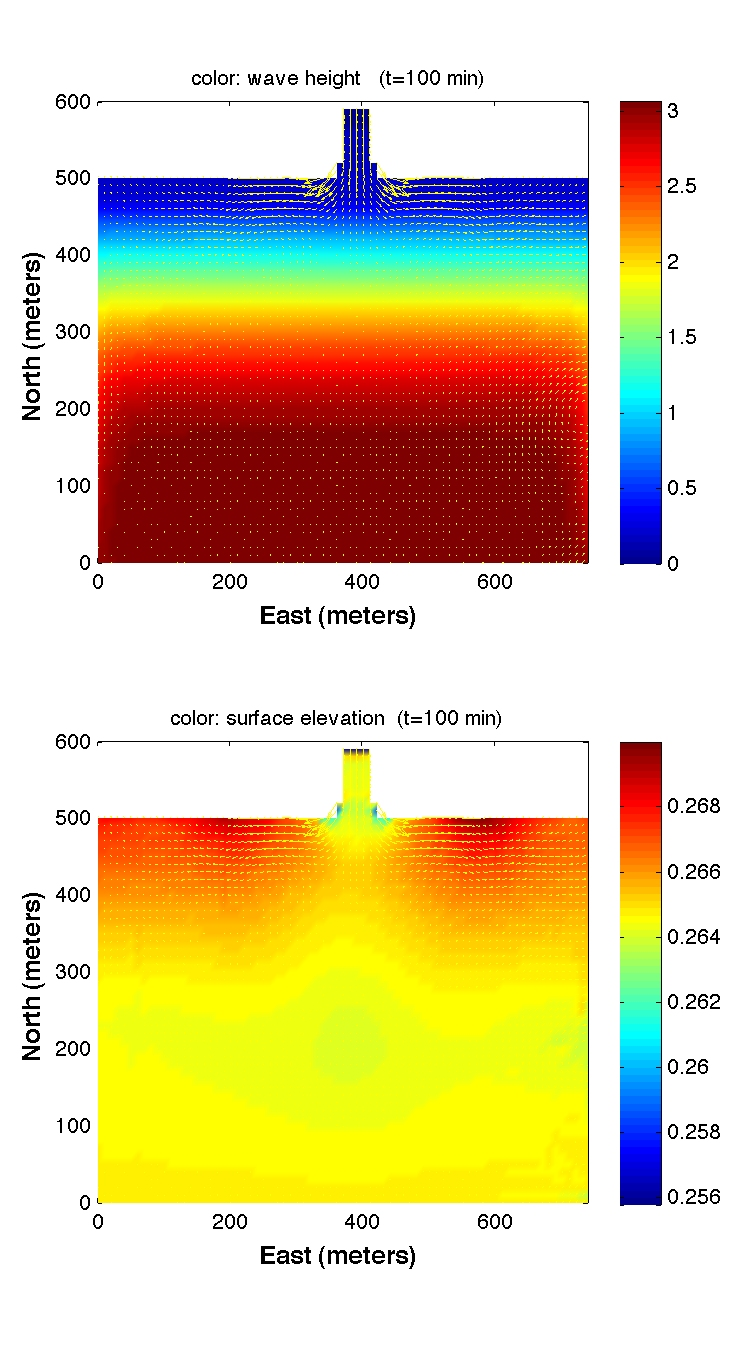
\includegraphics[width=0.8\textwidth]{../figures/ideal_100min.jpg}
	\caption{(Top panel) wave height (color) and currents. (Bottom panel) surface elevation (color) and currents.}
	\label{ideal_result}
\end{figure}

The model grid is generated with dx=dy=10 m and a dimension of 80 x 60. The grid generation file is provided in /input/ mkxyz.f. mkxyz produces x\_circ.txt, y\_circ.txt, and dep\_circ.txt for SHORECIRC, and xxyy\_swan.txt and dep\_swan.txt for SWAN. Note that, in the test case, SWAN and SHORECIRC use the same grid, meaning that the coordinates (x,y) for the both models are the same. For a general application, the SWAN grid and SHORECIRC grid can be different. 

The test needs a time series of wave for SWAN, tidal and river conditions for SHORECIRC. They are generated by programs:  mk\_wave\_constant.m, mk\_tide.f90 and mk\_river.f90, respectively, provided in /input/. mk\_wave\_constant.m generated time series of wave spectrum parameters saved in wave.txt. mk\_tide.f90 generates tidal constituents at every tidal boundary points, saved in tide.txt. mk\_river.f90 makes a time series of river flux at river boundary points, saved in river.txt.
 
The specific model configurations are listed below.

\begin{description}

\item {\bf SWAN INPUT}

SET 0 90 0.05 200 3 9.81 1025 0 0.10 CARTESIAN       
                                               
MODE NONSTATIONARY TWODIMENSIONAL                                                                   
                                                                                                
CGRID CURV 79 59 EXC -99999.0 -99999.0 CIRCLE 36 0.038 0.5 43         
                            
READGRID COOR 1 '{\bf ../input/xxyy\_swan.txt'} 3                                                                          
                                                                                                  
INPGRID BOTTOM CURV 0. 0. 79 59 EXC -99999.0              
                                        
READINP BOTTOM 1 '{\bf ../input/dep\_swan.txt'} 3 0 FREE                                                              
                                                                                                               
WIND 0 150                                                      
                                    
BOUNDPAR1 SHAPESPEC JONSWP 3.3 PEAK DSPR DEGREES         
                                           
BOUNDPAR2 SEGMENT IJ 0 0 79 0 CONSTANT FILE '{\bf ../input/wave.txt}'           
                                                                                                        
                                                                                     
WCAPping CSM               
                                                                         
BREAKING CONSTANT 1.0 0.73          
                                                                
FRICTION JON                                                                                        
                                                                                               
PROP BSBT                                                              
                             
NUMERIC ACCUR .02 .02 .02 98 STAT 15 0.0                                                            
                                                                                                                                                                                                                                                                                                                                                                                     
TEST 0,0                                       
                                                     
COMPUTE NONSTAT 20081114.160000 1 MI 20081114.230000          
                                     
STOP        

\item {\bf WAVE CURRENT INTERATION}

SWAN\_RUN = T

SHORECIRC\_RUN = T

WC\_BOUND\_WEST = 5

WC\_BOUND\_EAST = 5

WC\_BOUND\_SOUTH = 5

WC\_BOUND\_NORTH = 0

WC\_LAG = 1800.0

\item {\bf PARALLEL INFO}

PX = 2

PY = 2  

\item{\bf SHORECIRC INPUT}

DEPTH\_TYPE = DATA

DEPTH\_FILE = {\bf ../input/dep\_circ.txt}

RESULT\_FOLDER = /Users/tmp/

PLOT\_INTV = 120.0

PLOT\_INTV\_STATION = 10.0

SCREEN\_INTV = 120.0

CORI\_CONSTANT = T

LATITUDE = 34.1

X\_FILE = {\bf ../input/x\_circ.txt}

Y\_FILE = {\bf ../input/y\_circ.txt}

ETA\_CLAMPED = T

FLUX\_CLAMPED = T

TIDE\_FILE = {\bf ../input/tide.txt}

FLUX\_FILE = {\bf ../input/river.txt}

Cd = 0.0026

Time\_Scheme = Runge\_Kutta

HIGH\_ORDER = FOURTH

CONSTRUCTION = HLLC

CFL = 0.5

FroudeCap = 0.8

MinDepth=0.01

MinDepthFrc = 0.01

NumberStations = 0

DEPTH\_OUT = T

U = T

V = T

ETA = T

HS = T

MASK = T

\end{description}

Figure \ref{ideal_result} shows  wave height (color) and currents (top panel) and surface elevation (color) and currents (bottom panel) at t = 100 min. The figure was plotted using plot\_hs\_uv.m provided in /postprocessing/.


\subsection{Simulation of longshore currents}

\subsection{Appendix A: Extended form of tensor expression}


The pressure gradient term and other first-order tensor term can be easily transformed between the Cartesian and generalized curvilinear coordinates using (\ref{der}) and (\ref{der2}). The radiation stresses and shear stresses contain more terms after coordinate transformation. The example of transformation for shear stress terms is demonstrated below. 

$\tau_{\alpha\beta}$ in Cartesian coordinates can be expressed as
\be
\tau_{\alpha\beta} = \mu_t \left( \frac{\partial u_\alpha}{\partial x_\beta} +\frac{\partial u_\beta}{\partial x_\alpha} \right)
\ee
After coordinate transformation, 
\be
\tau_{\alpha\beta} = \mu_t \left( L^\gamma_\beta \frac{\partial u_\alpha}{\partial \xi^\gamma} + 
 L^\gamma_\alpha \frac{\partial u_\beta}{\partial \xi^\gamma}   \right)
 \label{trans}
\ee
For coding, the extended form of (\ref{trans}) can be written as
\be
\tau_{11} = 2 \mu_t (L^1_1 u_{\xi^1} + L^2_1 u_{\xi^2})
\ee
 \be
\tau_{12} =\tau_{21} =   \mu_t (L^1_2 u_{\xi^1} + L^2_2 u_{\xi^2} + L^1_1 u_{\xi^1} + L^1_2 u_{\xi^2} )
\ee
\be
\tau_{22} = 2 \mu_t (L^1_2 u_{\xi^1} + L^2_2 u_{\xi^2})
\ee
The shear stress terms can be written as
\be
 J \frac{\partial }{\partial x_\beta}(H \tau_{\alpha\beta}) = \frac{\partial}{\partial \xi^\gamma} (\tau_{\alpha\beta}J H L^\gamma_\beta) 
 = J L^\gamma_\beta \frac{\partial}{\partial \xi^\gamma} (H \tau_{\alpha\beta})
\ee

In the code, $L^\alpha_\beta$ is defined as $L_{\alpha\beta}$. To keep a consistency with the code, we use $L_{\alpha\beta}$ and $\xi_\alpha$ to represent $L^\alpha_\beta$ and $\xi^\alpha$, respectively, in the following extended expressions.

The shear stress terms in $x$ direction can be expressed as
\ba
 \nonumber
 &&
JL_{11} (H\tau_{11})_{\xi_1} + JL_{21} (H\tau_{11})_{\xi_2} +JL_{12} (H\tau_{12})_{\xi_1}+JL_{22} (H\tau_{12})_{\xi_2}   
   \\
 \nonumber
 &&
= J L_{11} \mu_t \left [  2 H L_{11} u_{\xi_1\xi_1}  +  2 u_{\xi_1}(HL_{11})_{\xi_1}
+2 H L_{21} u_{\xi_1\xi_2} +2 u_{\xi_2}(HL_{21})_{\xi_1} \right] 
   \\
 \nonumber
 &&
 + J L_{12} \mu_t \left [  2 H L_{11} u_{\xi_1\xi_2}  +  2 u_{\xi_1}(HL_{11})_{\xi_2}
+2 H L_{21} u_{\xi_2\xi_2} +2 u_{\xi_2}(HL_{21})_{\xi_2} \right] 
   \\
 \nonumber
 &&
  + J L_{12} \mu_t \left [   H L_{12} u_{\xi_1\xi_1}  +   u_{\xi_1}(HL_{12})_{\xi_1}
+ H L_{22} u_{\xi_1\xi_2} + u_{\xi_2}(HL_{22})_{\xi_1} \right. 
   \\
 \nonumber
 &&  \ \ \ \  \ \ \ \ \ \ \ \ \ \ \ 
   +  \left.   H L_{11} v_{\xi_1\xi_1}  +   v_{\xi_1}(HL_{11})_{\xi_1}
+ H L_{12} v_{\xi_1\xi_2} + v_{\xi_2}(HL_{12})_{\xi_1} \right]
   \\
 \nonumber
 &&
  + J L_{22} \mu_t \left [   H L_{12} u_{\xi_1\xi_2}  +   u_{\xi_1}(HL_{12})_{\xi_2}
+ H L_{22} u_{\xi_2\xi_2} + u_{\xi_2}(HL_{22})_{\xi_2} \right. 
  \\
 && \ \ \ \  \ \ \ \ \ \ \ \ \ \ \ 
    +  \left.   H L_{11} v_{\xi_1\xi_2}  +   v_{\xi_1}(HL_{11})_{\xi_2}
+ H L_{12} v_{\xi_2\xi_2} + v_{\xi_2}(HL_{12})_{\xi_2} \right]
\ea
 in $y$ direction,
 \ba
 \nonumber
 &&
JL_{11} (H\tau_{21})_{\xi_1} + JL_{21} (H\tau_{21})_{\xi_2} +JL_{12} (H\tau_{22})_{\xi_1}+JL_{22} (H\tau_{22})_{\xi_2}   
   \\
 \nonumber
 &&
= J L_{22} \mu_t \left [  2 H L_{12} v_{\xi_1\xi_2}  +  2 v_{\xi_1}(HL_{12})_{\xi_2}
+2 H L_{22} v_{\xi_2\xi_2} +2 v_{\xi_2}(HL_{22})_{\xi_2} \right] 
   \\
 \nonumber
 &&
 + J L_{12} \mu_t \left [  2 H L_{12} v_{\xi_1\xi_1}  +  2 v_{\xi_1}(HL_{12})_{\xi_1}
+2 H L_{22} v_{\xi_1\xi_2} +2 v_{\xi_2}(HL_{22})_{\xi_1} \right] 
   \\
 \nonumber
 &&
  + J L_{12} \mu_t \left [   H L_{12} u_{\xi_1\xi_2}  +   u_{\xi_1}(HL_{12})_{\xi_2}
+ H L_{22} u_{\xi_2 \xi_2} + u_{\xi_2}(HL_{22})_{\xi_2} \right. 
   \\
 \nonumber
 &&  \ \ \ \  \ \ \ \ \ \ \ \ \ \ \ 
   +  \left.   H L_{11} v_{\xi_1\xi_2}  +   v_{\xi_1}(HL_{11})_{\xi_2}
+ H L_{12} v_{\xi_2\xi_2} + v_{\xi_2}(HL_{12})_{\xi_2} \right]
   \\
 \nonumber
 &&
  + J L_{11} \mu_t \left [   H L_{12} u_{\xi_1\xi_1}  +   u_{\xi_1}(HL_{12})_{\xi_1}
+ H L_{22} u_{\xi_1\xi_2} + u_{\xi_2}(HL_{22})_{\xi_1} \right. 
  \\
 && \ \ \ \  \ \ \ \ \ \ \ \ \ \ \ 
    +  \left.   H L_{11} v_{\xi_1\xi_1}  +   v_{\xi_1}(HL_{11})_{\xi_1}
+ H L_{12} v_{\xi_1\xi_2} + v_{\xi_2}(HL_{12})_{\xi_1} \right]
\ea

 

\section{References}

\begin{description}

\item Casulli, V. and Cheng, R. T., 1992, ``Semi-implicit finite difference methods for three-dimensional shallow water flow", {\em Int. J. Numer. Method Fluid}, 15 (6), 629-648. 

\item Erduran, K. S., Ilic, S., and Kutija, V., 2005, ``Hybrid finite-volume finite-difference scheme for the solution of Boussinesq equations", {\em Int. J. Numer. Meth. Fluid.}, 49, 1213-1232.

\item Gottlieb, S., Shu C.-W., and Tadmore, E., 2001, ``Strong stability-preserving high-order time discretization methods", {\em SIAM Review}, {\bf 43} (1), 89 - 112.

\item Haas, K. A., I. A. Svendsen, M. C. Haller, and Q. Zhao, 2003,
Quasi-three-dimensional modeling of rip current systems, {\em J. Geophys. Res.},
108, C7, 3216, doi:10.1029/2001JC001313.

\item Kim D. H., Cho, Y. S., and Kim, H. J., 2008, ``Well-balanced scheme between flux and source terms for computation of shallow-water equations over irregular bathymetry", {\em Journal of Engineering Mechanics}, 134, 277-290.

\item Kim, D. H., Lynett, P. J. and Socolofsky, S. A., 2009, ``A depth-integrated model for weakly dispersive, turbulent, and rotational
fluid flows'', {\em Ocean Modeling}, {\bf 27}, 198-214.

\item Kim, D. H., 2009, ``Turbulent flow and transport modeling by long waves and currents'', Ph.D. dissertation, Texas A\& M University.

\item Kirby, J. T., Wei, G., Chen, Q., Kennedy, A. B. and Dalrymple, R. A., 1998,  ``FUNWAVE 1.0, Fully nonlinear Boussinesq wave model. Documentation and user�s manual". Report CACR-98-06, Center for Applied Coastal Research, Department of Civil and Environmental Engineering, University of Delaware.

\item Kirby, J. T. and Dalrymple, R. A., 1992, "Combined Refraction/Diffraction Model REF/DIF 1, Version 2.4. Documentation and User's Manual", Research Report No. CACR-92-04, Center for Applied Coastal Research, Department of Civil Engineering, University of Delaware, Newark. 

\item Kirby, J. T., Shi, F., Harris, J. C., and Grilli, S. T., 2011, ``Sensitivity analysis of trans-oceanic tsunami propagation to dispersive and Coriolis effects", in preparation.  


\item Lynett, P. J., Wu, T.-R. and Liu, P. L.-F., 2002,  ``Modeling wave runup with depth-integrated equations",  {\em Coastal Engineering},  
46, 89-107.

\item Naik, N. H., Naik, V. K., and Nicoules, M., 1993, ``Parallelization of a class of implicit finite difference schemes in computational fluid dynamics", {\em  International Journal of High Speed Computing},  5: 1-50.

\item Newberger, P. A. and Allen, J. S., 2007, Forcing a three-dimensional, hydrostatic,
primitive-equation model for application in the surf zone:
1. Formulation, {\em J. Geophy. Res.}, 112, C08018, doi: 10.1029/2006JC003472

\item Ning, D. Z., Zang, J., Liang, Q., Taylor, P. H., and Borthwick, A. G. L., 2008, ``Boussinesq cut-cell model for non-linear wave interaction with coastal structures", {\em International Journal for Numerical Methods in Fluids}, 57 (10), 1459-1483.


\item Putrevu, U. and I. A. Svendsen, 1999, Three-dimensional dispersion of
momentum in wave-induced nearshore currents, {\em Eur. J. Mech. B/Fluids},
83-101.

\item Roeber, V., Cheung, K. F., and Kobayashi, M. H., 2010, ``Shock-capturing Boussinesq-type model for nearshore wave processes", {\em Coastal Engineering}, 57, 407-423.

\item Rogers, B. D., Borthwick, A. G. L., and Taylor, P. H., 2003, ``Mathematical balancing of flux gradient and source terms prior to using Roe's approximate Riemann solver", {\em Journal of Computational Physics}, 192, 422-451.

\item Shi, F., Kirby, J. T., Newberger, P. and Haas, K., 2005, "NearCoM masetr program for nearshore community model, Version 2005.4 - Documentation and user's manual", Research Report No. CACR-05-10, Center for Applied Coastal Research, Dept. of Civil and Environmental Engineering, Univ. of Delaware, Newark. 

\item Shi, F., Kirby, J. T., Tehranirad, B. and Harris, J. C., 2011a, FUNWAVE-TVD, users' manual and benchmark tests, Center for Applied Coastal Research Report, CACR 2011-04, University of Delaware, Newark, Delaware. 

\item Shi, F., Kirby, J. T., Harris, J. C., Geiman, J. D., and Grilli, S. T., 2011b, ``A high-order adaptive time-stepping TVD solver for Boussinesq modeling of breaking waves and coastal inundation",  {\em Ocean Modelling},  doi:10.1016/j.ocemod.2011.12.004.

\item Shi, F., Sun, W. and Wei, G., 1998, A WDM method on generalized curvilinear grid for calculation of storm
surge flooding, {\em Applied Ocean Research}, 19(4), 275-282.

\item Shi, F. and Sun, W., 1995, A variable boundary model of storm surge flooding in generalized curvilinear grids,  {\em International Journal for Numerical Methods in Fluids}, 21 (8), 642-651. 

\item Shi,F.,Svendsen,I.A., Kirby, J.T., and Smith, J. M., 2003, A curvilinear version of a Quasi-3D nearshore
circulation model, {\em Coastal Engineering}, 49 (1-2), 99-124

\item Shiach, J. B. and Mingham, C. G., 2009, ``A temporally second-order accurate Godunov-type scheme for solving the extended Boussinesq equations", {\em Coastal Engineering}, 56, 32-45.

\item Sitanggang, K. I. and Lynett, P., 2005, ``Parallel computation of a highly nonlinear Boussinesq equation model through domain
decomposition'', {\em Int. J. Num. Meth. Fluids}, {\bf 49}, 57-74.

\item Smagorinsky, J., 1963, ``General circulation experiments with the primitive equations. I. The basic experiment",  {\em Mon. Weather Rev}, 91, 99-165.

\item Svendsen I. A., K. A. Haas, and Q. Zhao, 2004, Quasi-3D Nearshore Circulation
Model SHORECIRC: Version 2.0, Research Report, Center for Applied
Coastal Research, University of Delaware.

\item Tehranirad, B., Shi, F., Kirby, J. T., Harris, J. C. and Grilli, S., 2011, ``Tsunami benchmark results for fully nonlinear Boussinesq wave model FUNWAVE-TVD, Version 1.0'', Research Report No. CACR-11-02, Center for Applied Coastal Research, University of Delaware.  

\item Tonelli, M. and Petti, M., 2009, ``Hybrid finite volume - finite difference scheme for 2DH improved Boussinesq equations'', {\em Coast. Engrng.}, {\bf 56}, 609-620.

\item Tonelli, M. and Petti, M., 2010, ``Finite volume scheme for the solution of 2D extended Boussinesq equations in the surf zone'', {\em Ocean Engrng.}, {\bf 37}, 567-582.

\item Toro, E. F., 2009, {\em Riemann solvers and numerical methods for fluid dynamics: a practical introduction}, Third edition, Springer, New York. 

\item
Yamamoto, S., Daiguji, H., 1993, ``Higher-order-accurate upwind schemes for solving 
the compressible Euler and Navier�Stokes equations", {\em Computers and Fluids},  22 
(2/3), 259�270. 

\item Yamamoto, S., Kano, S. and Daiguji, H, 1998, ``An efficient CFD approach for simulating unsteady hypersonic shock�shock interference flows", {\em Computers and Fluids} 27 (5�6), pp. 571-580. 

\item Zhou, J. G., Causon, D. M., Mingham C. G., and Ingram, D. M., 2001, ``The surface gradient method for the treatment of source terms in the shallow-water equations", {\em Journal of Computational Physics}, 168, 1-25.

\end{description}

%\begin{figure}[htbp]
%	\centering
%		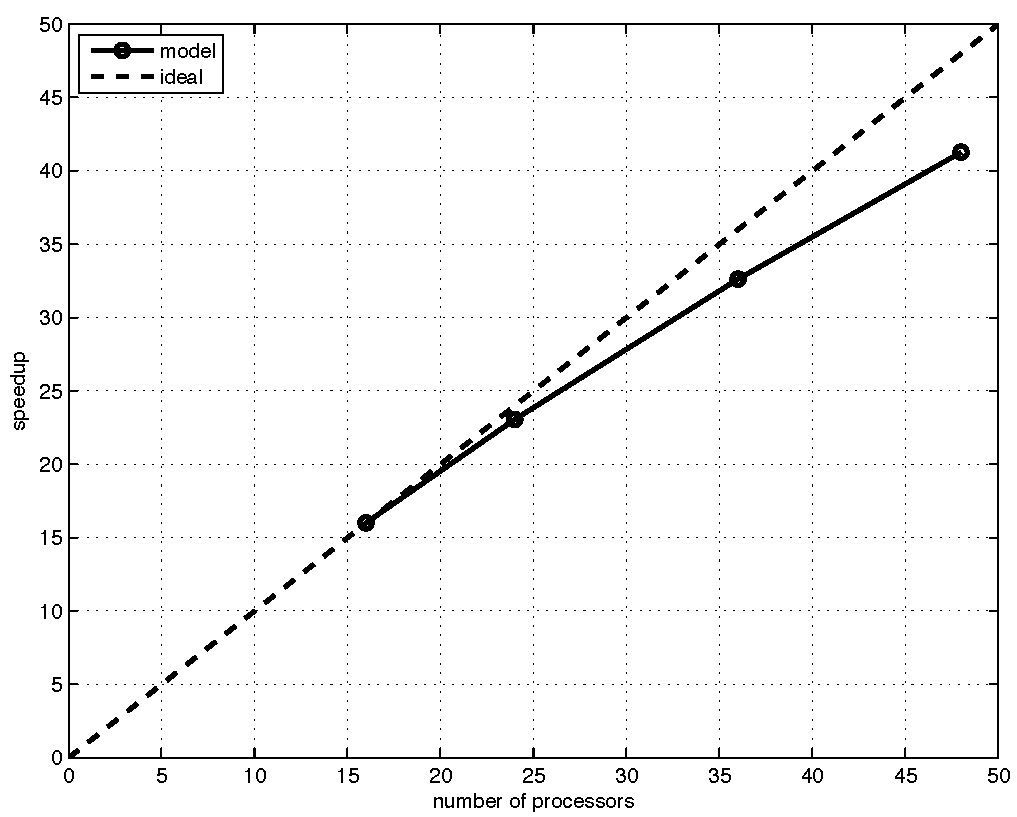
\includegraphics[width=0.8\textwidth]{../figures/speedup.JPG}
%	\caption{Variation in model performance with number of processors for a 5400 x 3600 domain.  Straight line indicates arithmetic speedup. Actual performance is shown in the curved line.}
%	\label{parallel}
%\end{figure}


\end{document}  